% Options for packages loaded elsewhere
\PassOptionsToPackage{unicode}{hyperref}
\PassOptionsToPackage{hyphens}{url}
\PassOptionsToPackage{dvipsnames,svgnames,x11names}{xcolor}
%
\documentclass[
  letterpaper,
  DIV=11,
  numbers=noendperiod]{scrartcl}

\usepackage{amsmath,amssymb}
\usepackage{iftex}
\ifPDFTeX
  \usepackage[T1]{fontenc}
  \usepackage[utf8]{inputenc}
  \usepackage{textcomp} % provide euro and other symbols
\else % if luatex or xetex
  \usepackage{unicode-math}
  \defaultfontfeatures{Scale=MatchLowercase}
  \defaultfontfeatures[\rmfamily]{Ligatures=TeX,Scale=1}
\fi
\usepackage{lmodern}
\ifPDFTeX\else  
    % xetex/luatex font selection
\fi
% Use upquote if available, for straight quotes in verbatim environments
\IfFileExists{upquote.sty}{\usepackage{upquote}}{}
\IfFileExists{microtype.sty}{% use microtype if available
  \usepackage[]{microtype}
  \UseMicrotypeSet[protrusion]{basicmath} % disable protrusion for tt fonts
}{}
\makeatletter
\@ifundefined{KOMAClassName}{% if non-KOMA class
  \IfFileExists{parskip.sty}{%
    \usepackage{parskip}
  }{% else
    \setlength{\parindent}{0pt}
    \setlength{\parskip}{6pt plus 2pt minus 1pt}}
}{% if KOMA class
  \KOMAoptions{parskip=half}}
\makeatother
\usepackage{xcolor}
\setlength{\emergencystretch}{3em} % prevent overfull lines
\setcounter{secnumdepth}{5}
% Make \paragraph and \subparagraph free-standing
\makeatletter
\ifx\paragraph\undefined\else
  \let\oldparagraph\paragraph
  \renewcommand{\paragraph}{
    \@ifstar
      \xxxParagraphStar
      \xxxParagraphNoStar
  }
  \newcommand{\xxxParagraphStar}[1]{\oldparagraph*{#1}\mbox{}}
  \newcommand{\xxxParagraphNoStar}[1]{\oldparagraph{#1}\mbox{}}
\fi
\ifx\subparagraph\undefined\else
  \let\oldsubparagraph\subparagraph
  \renewcommand{\subparagraph}{
    \@ifstar
      \xxxSubParagraphStar
      \xxxSubParagraphNoStar
  }
  \newcommand{\xxxSubParagraphStar}[1]{\oldsubparagraph*{#1}\mbox{}}
  \newcommand{\xxxSubParagraphNoStar}[1]{\oldsubparagraph{#1}\mbox{}}
\fi
\makeatother

\usepackage{color}
\usepackage{fancyvrb}
\newcommand{\VerbBar}{|}
\newcommand{\VERB}{\Verb[commandchars=\\\{\}]}
\DefineVerbatimEnvironment{Highlighting}{Verbatim}{commandchars=\\\{\}}
% Add ',fontsize=\small' for more characters per line
\usepackage{framed}
\definecolor{shadecolor}{RGB}{241,243,245}
\newenvironment{Shaded}{\begin{snugshade}}{\end{snugshade}}
\newcommand{\AlertTok}[1]{\textcolor[rgb]{0.68,0.00,0.00}{#1}}
\newcommand{\AnnotationTok}[1]{\textcolor[rgb]{0.37,0.37,0.37}{#1}}
\newcommand{\AttributeTok}[1]{\textcolor[rgb]{0.40,0.45,0.13}{#1}}
\newcommand{\BaseNTok}[1]{\textcolor[rgb]{0.68,0.00,0.00}{#1}}
\newcommand{\BuiltInTok}[1]{\textcolor[rgb]{0.00,0.23,0.31}{#1}}
\newcommand{\CharTok}[1]{\textcolor[rgb]{0.13,0.47,0.30}{#1}}
\newcommand{\CommentTok}[1]{\textcolor[rgb]{0.37,0.37,0.37}{#1}}
\newcommand{\CommentVarTok}[1]{\textcolor[rgb]{0.37,0.37,0.37}{\textit{#1}}}
\newcommand{\ConstantTok}[1]{\textcolor[rgb]{0.56,0.35,0.01}{#1}}
\newcommand{\ControlFlowTok}[1]{\textcolor[rgb]{0.00,0.23,0.31}{\textbf{#1}}}
\newcommand{\DataTypeTok}[1]{\textcolor[rgb]{0.68,0.00,0.00}{#1}}
\newcommand{\DecValTok}[1]{\textcolor[rgb]{0.68,0.00,0.00}{#1}}
\newcommand{\DocumentationTok}[1]{\textcolor[rgb]{0.37,0.37,0.37}{\textit{#1}}}
\newcommand{\ErrorTok}[1]{\textcolor[rgb]{0.68,0.00,0.00}{#1}}
\newcommand{\ExtensionTok}[1]{\textcolor[rgb]{0.00,0.23,0.31}{#1}}
\newcommand{\FloatTok}[1]{\textcolor[rgb]{0.68,0.00,0.00}{#1}}
\newcommand{\FunctionTok}[1]{\textcolor[rgb]{0.28,0.35,0.67}{#1}}
\newcommand{\ImportTok}[1]{\textcolor[rgb]{0.00,0.46,0.62}{#1}}
\newcommand{\InformationTok}[1]{\textcolor[rgb]{0.37,0.37,0.37}{#1}}
\newcommand{\KeywordTok}[1]{\textcolor[rgb]{0.00,0.23,0.31}{\textbf{#1}}}
\newcommand{\NormalTok}[1]{\textcolor[rgb]{0.00,0.23,0.31}{#1}}
\newcommand{\OperatorTok}[1]{\textcolor[rgb]{0.37,0.37,0.37}{#1}}
\newcommand{\OtherTok}[1]{\textcolor[rgb]{0.00,0.23,0.31}{#1}}
\newcommand{\PreprocessorTok}[1]{\textcolor[rgb]{0.68,0.00,0.00}{#1}}
\newcommand{\RegionMarkerTok}[1]{\textcolor[rgb]{0.00,0.23,0.31}{#1}}
\newcommand{\SpecialCharTok}[1]{\textcolor[rgb]{0.37,0.37,0.37}{#1}}
\newcommand{\SpecialStringTok}[1]{\textcolor[rgb]{0.13,0.47,0.30}{#1}}
\newcommand{\StringTok}[1]{\textcolor[rgb]{0.13,0.47,0.30}{#1}}
\newcommand{\VariableTok}[1]{\textcolor[rgb]{0.07,0.07,0.07}{#1}}
\newcommand{\VerbatimStringTok}[1]{\textcolor[rgb]{0.13,0.47,0.30}{#1}}
\newcommand{\WarningTok}[1]{\textcolor[rgb]{0.37,0.37,0.37}{\textit{#1}}}

\providecommand{\tightlist}{%
  \setlength{\itemsep}{0pt}\setlength{\parskip}{0pt}}\usepackage{longtable,booktabs,array}
\usepackage{calc} % for calculating minipage widths
% Correct order of tables after \paragraph or \subparagraph
\usepackage{etoolbox}
\makeatletter
\patchcmd\longtable{\par}{\if@noskipsec\mbox{}\fi\par}{}{}
\makeatother
% Allow footnotes in longtable head/foot
\IfFileExists{footnotehyper.sty}{\usepackage{footnotehyper}}{\usepackage{footnote}}
\makesavenoteenv{longtable}
\usepackage{graphicx}
\makeatletter
\newsavebox\pandoc@box
\newcommand*\pandocbounded[1]{% scales image to fit in text height/width
  \sbox\pandoc@box{#1}%
  \Gscale@div\@tempa{\textheight}{\dimexpr\ht\pandoc@box+\dp\pandoc@box\relax}%
  \Gscale@div\@tempb{\linewidth}{\wd\pandoc@box}%
  \ifdim\@tempb\p@<\@tempa\p@\let\@tempa\@tempb\fi% select the smaller of both
  \ifdim\@tempa\p@<\p@\scalebox{\@tempa}{\usebox\pandoc@box}%
  \else\usebox{\pandoc@box}%
  \fi%
}
% Set default figure placement to htbp
\def\fps@figure{htbp}
\makeatother
% definitions for citeproc citations
\NewDocumentCommand\citeproctext{}{}
\NewDocumentCommand\citeproc{mm}{%
  \begingroup\def\citeproctext{#2}\cite{#1}\endgroup}
\makeatletter
 % allow citations to break across lines
 \let\@cite@ofmt\@firstofone
 % avoid brackets around text for \cite:
 \def\@biblabel#1{}
 \def\@cite#1#2{{#1\if@tempswa , #2\fi}}
\makeatother
\newlength{\cslhangindent}
\setlength{\cslhangindent}{1.5em}
\newlength{\csllabelwidth}
\setlength{\csllabelwidth}{3em}
\newenvironment{CSLReferences}[2] % #1 hanging-indent, #2 entry-spacing
 {\begin{list}{}{%
  \setlength{\itemindent}{0pt}
  \setlength{\leftmargin}{0pt}
  \setlength{\parsep}{0pt}
  % turn on hanging indent if param 1 is 1
  \ifodd #1
   \setlength{\leftmargin}{\cslhangindent}
   \setlength{\itemindent}{-1\cslhangindent}
  \fi
  % set entry spacing
  \setlength{\itemsep}{#2\baselineskip}}}
 {\end{list}}
\usepackage{calc}
\newcommand{\CSLBlock}[1]{\hfill\break\parbox[t]{\linewidth}{\strut\ignorespaces#1\strut}}
\newcommand{\CSLLeftMargin}[1]{\parbox[t]{\csllabelwidth}{\strut#1\strut}}
\newcommand{\CSLRightInline}[1]{\parbox[t]{\linewidth - \csllabelwidth}{\strut#1\strut}}
\newcommand{\CSLIndent}[1]{\hspace{\cslhangindent}#1}

\KOMAoption{captions}{tableheading}
\makeatletter
\@ifpackageloaded{caption}{}{\usepackage{caption}}
\AtBeginDocument{%
\ifdefined\contentsname
  \renewcommand*\contentsname{Table of contents}
\else
  \newcommand\contentsname{Table of contents}
\fi
\ifdefined\listfigurename
  \renewcommand*\listfigurename{List of Figures}
\else
  \newcommand\listfigurename{List of Figures}
\fi
\ifdefined\listtablename
  \renewcommand*\listtablename{List of Tables}
\else
  \newcommand\listtablename{List of Tables}
\fi
\ifdefined\figurename
  \renewcommand*\figurename{Figure}
\else
  \newcommand\figurename{Figure}
\fi
\ifdefined\tablename
  \renewcommand*\tablename{Table}
\else
  \newcommand\tablename{Table}
\fi
}
\@ifpackageloaded{float}{}{\usepackage{float}}
\floatstyle{ruled}
\@ifundefined{c@chapter}{\newfloat{codelisting}{h}{lop}}{\newfloat{codelisting}{h}{lop}[chapter]}
\floatname{codelisting}{Listing}
\newcommand*\listoflistings{\listof{codelisting}{List of Listings}}
\makeatother
\makeatletter
\makeatother
\makeatletter
\@ifpackageloaded{caption}{}{\usepackage{caption}}
\@ifpackageloaded{subcaption}{}{\usepackage{subcaption}}
\makeatother

\usepackage{bookmark}

\IfFileExists{xurl.sty}{\usepackage{xurl}}{} % add URL line breaks if available
\urlstyle{same} % disable monospaced font for URLs
\hypersetup{
  pdftitle={Resilience of Public Transportation Networks},
  colorlinks=true,
  linkcolor={blue},
  filecolor={Maroon},
  citecolor={Blue},
  urlcolor={Blue},
  pdfcreator={LaTeX via pandoc}}


\title{Resilience of Public Transportation Networks}
\usepackage{etoolbox}
\makeatletter
\providecommand{\subtitle}[1]{% add subtitle to \maketitle
  \apptocmd{\@title}{\par {\large #1 \par}}{}{}
}
\makeatother
\subtitle{UGE: M2 SIA - NetRes Project Report}
\author{Luca Uckermann}
\date{2025-02-02}

\begin{document}
\maketitle
\begin{abstract}
This report examines the resilience of public transportation networks
using percolation theory to evaluate the impact of link and node
failures. Quality matrices based on metrics such as travel time and
betweenness centrality are used to simulate disruptions and assess the
network's ability to sustain passenger demand. The analysis reveals the
vulnerability of critical components and highlights the need for
strategic interventions such as strengthening high-centrality nodes and
links. The results provide actionable insights for designing robust
transportation systems capable of withstanding disruptions while
maintaining functionality.
\end{abstract}

\renewcommand*\contentsname{Table of contents}
{
\hypersetup{linkcolor=}
\setcounter{tocdepth}{2}
\tableofcontents
}

\section{Introduction}\label{introduction}

Public transportation networks are essential for enabling urban
mobility, connecting people to jobs, schools, health care, and other
essential services. However, these networks are vulnerable to
disruptions caused by congestion, accidents, maintenance issues, or
targeted attacks. Ensuring their resilience (the ability to maintain
functionality in the face of such disruptions) is a key priority for
city planners. Understanding the impact of disruptions and developing
strategies to mitigate them is critical to the design and management of
robust transportation systems.

Percolation theory provides a powerful and structured framework for
studying network resilience. By systematically removing components, such
as links or nodes, and analyzing the resulting changes in connectivity
and performance, percolation theory helps identify critical failure
points and assess the robustness of a network. Recent research by
Hamedmoghadam et al.~(2021) has extended the application of percolation
theory to heterogeneous flow demand in networks, emphasizing the
functional aspects of resilience alongside structural analysis
(\citeproc{ref-hamedmoghadam2021percolation}{Hamedmoghadam et al.
2021}). This approach provides a more nuanced understanding of network
performance under progressive disturbances, particularly in demand-side
systems such as public transportation.

This report builds on the work of Hamedmoghadam et al.~(2021) and
analyzes the resilience of a public transportation network under various
disruption scenarios. The study incorporates quality matrices based on
metrics such as travel time and betweenness centrality to evaluate the
impact of link and node removals on the network's ability to serve
passenger demand. By focusing on both structural connectivity and
functional performance, this research provides actionable insights into
network vulnerabilities and strategies to improve resilience.

This report is organized as follows: the next section introduces the
theoretical foundations of percolation theory, followed by the
development of quality matrices to quantify the performance of network
components. The main algorithm for simulating link and node failures is
then described, along with visualizations of the results. Finally, the
report concludes with practical recommendations for improving the
resilience of public transportation networks through strategic
interventions and resource allocation.

\section{Understanding the percolation
Theory}\label{understanding-the-percolation-theory}

\subsection{Definition}\label{definition}

Percolation theory is a powerful framework for studying how networks
maintain or lose connectivity and functionality as their components
(links or nodes) degrade or fail. This theoretical model is widely used
to evaluate the resilience of infrastructure networks, including
transportation systems, power grids, and communication networks.

In this study, the percolation process is modeled by progressively
removing network links based on their quality. Each link is assigned a
``quality'' metric, denoted as \(q_{ij} \in (0,1]\), which reflects its
relative performance. For example, in transportation networks,
\(q_{ij}\) may represent the ratio of the instantaneous travel speed to
the maximum allowable speed for a road segment.

The percolation process introduces a threshold \(\rho\), where all links
with \(q_{ij} \leq \rho\) are removed. This results in a subnetwork
\(G_\rho\) containing only links with quality above the threshold. By
systematically increasing \(\rho\) from \(0\) to \(1\), the network
transitions from global connectivity to fragmentation. A critical
threshold \(\rho_c\) emerges, indicating the point at which the largest
connected component (the \emph{giant component}, or \emph{GC})
disintegrates into smaller, disconnected clusters. This critical
threshold is a fundamental indicator of network robustness because it
marks the loss of overall connectivity.

While traditional percolation models focus on structural connectivity
(i.e., the topological configuration of networks), this work extends
this approach by incorporating heterogeneous flow demand. This
recognizes that in demand-driven networks such as public transportation,
passenger or data flow between origin-destination (O-D) pairs is not
evenly distributed. Even after the giant component collapses, a
significant portion of the demand may still be feasible if critical
paths persist within the fragmented network.

Two metrics are introduced to evaluate network performance during the
percolation process:

\begin{enumerate}
\def\labelenumi{\arabic{enumi}.}
\tightlist
\item
  \textbf{Unaffected Demand (UD):} The fraction of flow demand that
  remains feasible when links are removed.
\item
  \textbf{Reliability Metric (\(\alpha\)):} The area under the
  unaffected demand curve plotted against the threshold \(\rho\). This
  provides a comprehensive measure of the network's ability to sustain
  flow demand during the degradation process.
\end{enumerate}

By combining structural analysis with flow dynamics, percolation theory
enables the identification of critical links (bottlenecks) whose failure
significantly impacts network performance. This holistic perspective
informs strategic interventions to improve the connectivity and
reliability of critical infrastructure systems.

\subsection{Relevance}\label{relevance}

Percolation theory is essential for understanding and improving the
resilience of networks, particularly in the face of disruptions or
failures. The resilience of a network refers to its ability to maintain
functionality under adverse conditions, such as targeted attacks or
natural degradation.

This framework models disruptions by assigning a quality metric to each
link and progressively removing links below a specified threshold. By
simulating this systematic degradation, it is possible to evaluate:

\begin{itemize}
\tightlist
\item
  \textbf{Network Vulnerability:} The rate at which connectivity and
  functionality are lost as components fail.
\item
  \textbf{Critical Thresholds:} The points at which global connectivity
  or demand flow becomes unsustainable.
\end{itemize}

In infrastructure systems such as transportation or communication
networks, disruptions can result from congestion, accidents, natural
disasters, or targeted attacks. Percolation theory provides a structured
way to evaluate how these disruptions affect the network. The critical
threshold \(\rho_c\) serves as a key indicator of network robustness.

A key strength of this theory is its ability to incorporate both
structural and functional aspects of resilience:

\begin{enumerate}
\def\labelenumi{\arabic{enumi}.}
\tightlist
\item
  \textbf{Structural Analysis:} Examines how the removal of links or
  nodes affects the topological connectivity.
\item
  \textbf{Flow Dynamics:} Evaluates how disruptions affect the network's
  ability to support flows (e.g., passenger movement, data transfer).
\end{enumerate}

This study's focus on heterogeneous flow demand highlights the
importance of resilience beyond structural connectivity. While global
connectivity may collapse at a critical threshold, a significant portion
of flow demand may still be served by smaller, high-quality subnetworks.
This distinction is essential for real-world applications, where
maintaining service for critical flows is often more important than
maintaining full connectivity.

In addition, percolation theory makes it possible to identify bottleneck
components-critical links or nodes whose failure disproportionately
affects network functionality. Targeted interventions, such as
increasing redundancy or hardening these bottlenecks, can significantly
improve resilience. For example, in a public transportation network,
bottleneck analysis can guide investments to increase capacity, improve
connectivity, or reduce vulnerability.

In summary, percolation theory provides a comprehensive and practical
framework for assessing and improving the resilience of infrastructure
networks. By integrating structural and functional perspectives, it
provides valuable insights for designing robust systems that can
withstand and adapt to disruptions.

\section{Computing multiple quality
matrices}\label{computing-multiple-quality-matrices}

\subsection{Adjacency matrix}\label{adjacency-matrix}

The adjacency matrix (\(A\)) is a fundamental component for representing
a network. It encodes the connectivity between nodes, where each entry
\(A_{ij}\) indicates the presence or absence of a connection between
nodes \(i\) and \(j\). In this project, the adjacency matrix is
complemented by a weight matrix (\(w\)) that captures the travel time
along each link. Together, these matrices serve as the basis for
computing various quality metrics.

\begin{Shaded}
\begin{Highlighting}[]
\KeywordTok{function}\NormalTok{ [}\VariableTok{Adj}\OperatorTok{,} \VariableTok{wAdj}\NormalTok{] }\OperatorTok{=} \VariableTok{ComputeAdj2}\NormalTok{(}\VariableTok{ROUTES}\OperatorTok{,} \VariableTok{TravelLinkTime}\OperatorTok{,} \VariableTok{Stops}\NormalTok{)}
    \VariableTok{numStops} \OperatorTok{=} \VariableTok{length}\NormalTok{(}\VariableTok{Stops}\NormalTok{)}\OperatorTok{;}
    \VariableTok{Adj} \OperatorTok{=} \VariableTok{zeros}\NormalTok{(}\VariableTok{numStops}\OperatorTok{,} \VariableTok{numStops}\NormalTok{)}\OperatorTok{;}
    \VariableTok{wAdj} \OperatorTok{=} \VariableTok{zeros}\NormalTok{(}\VariableTok{numStops}\OperatorTok{,} \VariableTok{numStops}\NormalTok{)}\OperatorTok{;}

    \KeywordTok{for} \VariableTok{itinerary} \OperatorTok{=} \FloatTok{1}\OperatorTok{:}\VariableTok{size}\NormalTok{(}\VariableTok{ROUTES}\OperatorTok{,} \FloatTok{2}\NormalTok{)}
        \VariableTok{LastStopIdx} \OperatorTok{=} \VariableTok{find}\NormalTok{(}\VariableTok{strcmp}\NormalTok{(}\VariableTok{Stops}\OperatorTok{,} \VariableTok{ROUTES}\NormalTok{\{}\VariableTok{itinerary}\NormalTok{\}\{}\FloatTok{1}\NormalTok{\}))}\OperatorTok{;}

        \KeywordTok{for} \VariableTok{Stop} \OperatorTok{=} \FloatTok{2}\OperatorTok{:}\VariableTok{size}\NormalTok{(}\VariableTok{ROUTES}\NormalTok{\{}\VariableTok{itinerary}\NormalTok{\}}\OperatorTok{,} \FloatTok{2}\NormalTok{)}
            \VariableTok{StopIdx} \OperatorTok{=} \VariableTok{find}\NormalTok{(}\VariableTok{strcmp}\NormalTok{(}\VariableTok{Stops}\OperatorTok{,} \VariableTok{ROUTES}\NormalTok{\{}\VariableTok{itinerary}\NormalTok{\}\{}\VariableTok{Stop}\NormalTok{\}))}\OperatorTok{;}

            \VariableTok{Adj}\NormalTok{(}\VariableTok{LastStopIdx}\OperatorTok{,} \VariableTok{StopIdx}\NormalTok{) }\OperatorTok{=} \FloatTok{1}\OperatorTok{;}
            \VariableTok{wAdj}\NormalTok{(}\VariableTok{LastStopIdx}\OperatorTok{,} \VariableTok{StopIdx}\NormalTok{) }\OperatorTok{=} \VariableTok{TravelLinkTime}\NormalTok{\{}\VariableTok{itinerary}\NormalTok{\}\{}\VariableTok{Stop} \OperatorTok{{-}} \FloatTok{1}\NormalTok{\}}\OperatorTok{;}

            \VariableTok{LastStopIdx} \OperatorTok{=} \VariableTok{StopIdx}\OperatorTok{;}
        \KeywordTok{end}
    \KeywordTok{end}

    \VariableTok{Adj} \OperatorTok{=} \VariableTok{max}\NormalTok{(}\VariableTok{Adj}\OperatorTok{,} \VariableTok{Adj}\OperatorTok{\textquotesingle{}}\NormalTok{)}\OperatorTok{;}
    \VariableTok{wAdj} \OperatorTok{=} \VariableTok{max}\NormalTok{(}\VariableTok{wAdj}\OperatorTok{,} \VariableTok{wAdj}\OperatorTok{\textquotesingle{}}\NormalTok{)}\OperatorTok{;}
\KeywordTok{end}
\end{Highlighting}
\end{Shaded}

\begin{itemize}
\tightlist
\item
  \textbf{Input:}

  \begin{itemize}
  \tightlist
  \item
    ROUTES: A cell array specifying the sequence of stops for each
    route.
  \item
    TravelLinkTime: A cell array specifying the travel times between
    consecutive stops.
  \item
    Stops: A list of all stops in the network.
  \end{itemize}
\item
  \textbf{Outputs:}.

  \begin{itemize}
  \tightlist
  \item
    Adj: The adjacency matrix indicating the connectivity between stops.
  \item
    wAdj: The weight matrix representing the travel times between stops.
  \end{itemize}
\item
  \textbf{Key Features:}

  \begin{itemize}
  \tightlist
  \item
    The function handles directed and undirected networks by
    symmetrizing the matrices.
  \item
    The use of strcmp ensures robustness in matching stop names to their
    indices.
  \end{itemize}
\end{itemize}

\subsection{Quality matrix based on Travel
Time}\label{quality-matrix-based-on-travel-time}

Travel time is a critical factor in evaluating route quality. The
quality matrix (\(q\)) based on travel time assigns a quality score to
each link, where \(q_{ij} = \frac{1}{\text{TravelTime}_{ij}}\). Links
with shorter travel times are assigned higher quality scores, reflecting
their efficiency.

\begin{Shaded}
\begin{Highlighting}[]
\KeywordTok{function}\NormalTok{ [}\VariableTok{Adj}\OperatorTok{,} \VariableTok{wAdj}\OperatorTok{,} \VariableTok{qAdj}\NormalTok{] }\OperatorTok{=} \VariableTok{ComputeAdj2}\NormalTok{(}\VariableTok{ROUTES}\OperatorTok{,} \VariableTok{TravelLinkTime}\OperatorTok{,} \VariableTok{Stops}\NormalTok{)}
    \VariableTok{numStops} \OperatorTok{=} \VariableTok{length}\NormalTok{(}\VariableTok{Stops}\NormalTok{)}\OperatorTok{;}
    \VariableTok{Adj} \OperatorTok{=} \VariableTok{zeros}\NormalTok{(}\VariableTok{numStops}\OperatorTok{,} \VariableTok{numStops}\NormalTok{)}\OperatorTok{;}
    \VariableTok{wAdj} \OperatorTok{=} \VariableTok{zeros}\NormalTok{(}\VariableTok{numStops}\OperatorTok{,} \VariableTok{numStops}\NormalTok{)}\OperatorTok{;}
    \VariableTok{qAdj} \OperatorTok{=} \VariableTok{inf}\NormalTok{(}\VariableTok{numStops}\OperatorTok{,} \VariableTok{numStops}\NormalTok{)}\OperatorTok{;}

    \KeywordTok{for} \VariableTok{itinerary} \OperatorTok{=} \FloatTok{1}\OperatorTok{:}\VariableTok{size}\NormalTok{(}\VariableTok{ROUTES}\OperatorTok{,} \FloatTok{2}\NormalTok{)}
        \VariableTok{LastStopIdx} \OperatorTok{=} \VariableTok{find}\NormalTok{(}\VariableTok{strcmp}\NormalTok{(}\VariableTok{Stops}\OperatorTok{,} \VariableTok{ROUTES}\NormalTok{\{}\VariableTok{itinerary}\NormalTok{\}\{}\FloatTok{1}\NormalTok{\}))}\OperatorTok{;}

        \KeywordTok{for} \VariableTok{Stop} \OperatorTok{=} \FloatTok{2}\OperatorTok{:}\VariableTok{size}\NormalTok{(}\VariableTok{ROUTES}\NormalTok{\{}\VariableTok{itinerary}\NormalTok{\}}\OperatorTok{,} \FloatTok{2}\NormalTok{)}
            \VariableTok{StopIdx} \OperatorTok{=} \VariableTok{find}\NormalTok{(}\VariableTok{strcmp}\NormalTok{(}\VariableTok{Stops}\OperatorTok{,} \VariableTok{ROUTES}\NormalTok{\{}\VariableTok{itinerary}\NormalTok{\}\{}\VariableTok{Stop}\NormalTok{\}))}\OperatorTok{;}

            \VariableTok{Adj}\NormalTok{(}\VariableTok{LastStopIdx}\OperatorTok{,} \VariableTok{StopIdx}\NormalTok{) }\OperatorTok{=} \FloatTok{1}\OperatorTok{;}
            \VariableTok{wAdj}\NormalTok{(}\VariableTok{LastStopIdx}\OperatorTok{,} \VariableTok{StopIdx}\NormalTok{) }\OperatorTok{=} \VariableTok{TravelLinkTime}\NormalTok{\{}\VariableTok{itinerary}\NormalTok{\}\{}\VariableTok{Stop} \OperatorTok{{-}} \FloatTok{1}\NormalTok{\}}\OperatorTok{;}

            \KeywordTok{if} \VariableTok{TravelLinkTime}\NormalTok{\{}\VariableTok{itinerary}\NormalTok{\}\{}\VariableTok{Stop} \OperatorTok{{-}} \FloatTok{1}\NormalTok{\} }\OperatorTok{\textgreater{}} \FloatTok{0}
                \VariableTok{qAdj}\NormalTok{(}\VariableTok{LastStopIdx}\OperatorTok{,} \VariableTok{StopIdx}\NormalTok{) }\OperatorTok{=} \FloatTok{1} \OperatorTok{/} \VariableTok{TravelLinkTime}\NormalTok{\{}\VariableTok{itinerary}\NormalTok{\}\{}\VariableTok{Stop} \OperatorTok{{-}} \FloatTok{1}\NormalTok{\}}\OperatorTok{;}
            \KeywordTok{end}

            \VariableTok{LastStopIdx} \OperatorTok{=} \VariableTok{StopIdx}\OperatorTok{;}
        \KeywordTok{end}
    \KeywordTok{end}

    \VariableTok{Adj} \OperatorTok{=} \VariableTok{max}\NormalTok{(}\VariableTok{Adj}\OperatorTok{,} \VariableTok{Adj}\OperatorTok{\textquotesingle{}}\NormalTok{)}\OperatorTok{;}
    \VariableTok{wAdj} \OperatorTok{=} \VariableTok{max}\NormalTok{(}\VariableTok{wAdj}\OperatorTok{,} \VariableTok{wAdj}\OperatorTok{\textquotesingle{}}\NormalTok{)}\OperatorTok{;}
    \VariableTok{qAdj} \OperatorTok{=} \VariableTok{min}\NormalTok{(}\VariableTok{qAdj}\OperatorTok{,} \VariableTok{qAdj}\OperatorTok{\textquotesingle{}}\NormalTok{)}\OperatorTok{;}
\KeywordTok{end}
\end{Highlighting}
\end{Shaded}

\begin{itemize}
\tightlist
\item
  \textbf{Quality Metric:} Links with shorter travel times are assigned
  higher quality values, making \(q\) inversely proportional to travel
  time.
\item
  \textbf{Infinity Handling:} Initializing \(q\) with \(\infty\) ensures
  that unconnected links retain a high value, effectively excluding them
  from percolation calculations.
\item
  \textbf{Symmetry:} Quality values are symmetrized to ensure
  consistency across undirected links.
\end{itemize}

\subsection{Quality matrix based on inverse Travel
Time}\label{quality-matrix-based-on-inverse-travel-time}

The inverse travel time quality matrix normalizes \(q_{ij}\) by the
maximum observed travel time to ensure that all values are within
\((0,1]\). This metric highlights the relative efficiency of links.

\begin{Shaded}
\begin{Highlighting}[]
\KeywordTok{function}\NormalTok{ [}\VariableTok{Adj}\OperatorTok{,} \VariableTok{wAdj}\OperatorTok{,} \VariableTok{qAdj}\OperatorTok{,} \VariableTok{qInverseAdj}\NormalTok{] }\OperatorTok{=} \VariableTok{ComputeAdj2}\NormalTok{(}\VariableTok{ROUTES}\OperatorTok{,} \VariableTok{TravelLinkTime}\OperatorTok{,} \VariableTok{Stops}\NormalTok{)}
    \VariableTok{numStops} \OperatorTok{=} \VariableTok{length}\NormalTok{(}\VariableTok{Stops}\NormalTok{)}\OperatorTok{;}
    \VariableTok{Adj} \OperatorTok{=} \VariableTok{zeros}\NormalTok{(}\VariableTok{numStops}\OperatorTok{,} \VariableTok{numStops}\NormalTok{)}\OperatorTok{;}
    \VariableTok{wAdj} \OperatorTok{=} \VariableTok{zeros}\NormalTok{(}\VariableTok{numStops}\OperatorTok{,} \VariableTok{numStops}\NormalTok{)}\OperatorTok{;}
    \VariableTok{qAdj} \OperatorTok{=} \VariableTok{inf}\NormalTok{(}\VariableTok{numStops}\OperatorTok{,} \VariableTok{numStops}\NormalTok{)}\OperatorTok{;}
    \VariableTok{qInverseAdj} \OperatorTok{=} \VariableTok{inf}\NormalTok{(}\VariableTok{numStops}\OperatorTok{,} \VariableTok{numStops}\NormalTok{)}\OperatorTok{;}

    \KeywordTok{for} \VariableTok{itinerary} \OperatorTok{=} \FloatTok{1}\OperatorTok{:}\VariableTok{size}\NormalTok{(}\VariableTok{ROUTES}\OperatorTok{,} \FloatTok{2}\NormalTok{)}
        \VariableTok{LastStopIdx} \OperatorTok{=} \VariableTok{find}\NormalTok{(}\VariableTok{strcmp}\NormalTok{(}\VariableTok{Stops}\OperatorTok{,} \VariableTok{ROUTES}\NormalTok{\{}\VariableTok{itinerary}\NormalTok{\}\{}\FloatTok{1}\NormalTok{\}))}\OperatorTok{;}

        \KeywordTok{for} \VariableTok{Stop} \OperatorTok{=} \FloatTok{2}\OperatorTok{:}\VariableTok{size}\NormalTok{(}\VariableTok{ROUTES}\NormalTok{\{}\VariableTok{itinerary}\NormalTok{\}}\OperatorTok{,} \FloatTok{2}\NormalTok{)}
            \VariableTok{StopIdx} \OperatorTok{=} \VariableTok{find}\NormalTok{(}\VariableTok{strcmp}\NormalTok{(}\VariableTok{Stops}\OperatorTok{,} \VariableTok{ROUTES}\NormalTok{\{}\VariableTok{itinerary}\NormalTok{\}\{}\VariableTok{Stop}\NormalTok{\}))}\OperatorTok{;}

            \VariableTok{Adj}\NormalTok{(}\VariableTok{LastStopIdx}\OperatorTok{,} \VariableTok{StopIdx}\NormalTok{) }\OperatorTok{=} \FloatTok{1}\OperatorTok{;}
            \VariableTok{wAdj}\NormalTok{(}\VariableTok{LastStopIdx}\OperatorTok{,} \VariableTok{StopIdx}\NormalTok{) }\OperatorTok{=} \VariableTok{TravelLinkTime}\NormalTok{\{}\VariableTok{itinerary}\NormalTok{\}\{}\VariableTok{Stop} \OperatorTok{{-}} \FloatTok{1}\NormalTok{\}}\OperatorTok{;}

            \KeywordTok{if} \VariableTok{TravelLinkTime}\NormalTok{\{}\VariableTok{itinerary}\NormalTok{\}\{}\VariableTok{Stop} \OperatorTok{{-}} \FloatTok{1}\NormalTok{\} }\OperatorTok{\textgreater{}} \FloatTok{0}
                \VariableTok{qAdj}\NormalTok{(}\VariableTok{LastStopIdx}\OperatorTok{,} \VariableTok{StopIdx}\NormalTok{) }\OperatorTok{=} \FloatTok{1} \OperatorTok{/} \VariableTok{TravelLinkTime}\NormalTok{\{}\VariableTok{itinerary}\NormalTok{\}\{}\VariableTok{Stop} \OperatorTok{{-}} \FloatTok{1}\NormalTok{\}}\OperatorTok{;}
            \KeywordTok{end}

            \VariableTok{LastStopIdx} \OperatorTok{=} \VariableTok{StopIdx}\OperatorTok{;}
        \KeywordTok{end}
    \KeywordTok{end}

    \VariableTok{maxTravelTime} \OperatorTok{=} \VariableTok{max}\NormalTok{(}\VariableTok{wAdj}\NormalTok{(}\VariableTok{wAdj} \OperatorTok{\textgreater{}} \FloatTok{0}\NormalTok{)}\OperatorTok{,}\NormalTok{ []}\OperatorTok{,} \SpecialStringTok{\textquotesingle{}all\textquotesingle{}}\NormalTok{)}\OperatorTok{;}
    \KeywordTok{for} \VariableTok{i} \OperatorTok{=} \FloatTok{1}\OperatorTok{:}\VariableTok{numStops}
        \KeywordTok{for} \VariableTok{j} \OperatorTok{=} \FloatTok{1}\OperatorTok{:}\VariableTok{numStops}
            \KeywordTok{if} \VariableTok{wAdj}\NormalTok{(}\VariableTok{i}\OperatorTok{,} \VariableTok{j}\NormalTok{) }\OperatorTok{\textgreater{}} \FloatTok{0}
                \VariableTok{qInverseAdj}\NormalTok{(}\VariableTok{i}\OperatorTok{,} \VariableTok{j}\NormalTok{) }\OperatorTok{=} \FloatTok{1} \OperatorTok{/}\NormalTok{ (}\VariableTok{maxTravelTime} \OperatorTok{*} \VariableTok{wAdj}\NormalTok{(}\VariableTok{i}\OperatorTok{,} \VariableTok{j}\NormalTok{))}\OperatorTok{;}
            \KeywordTok{end}
        \KeywordTok{end}
    \KeywordTok{end}

    \VariableTok{Adj} \OperatorTok{=} \VariableTok{max}\NormalTok{(}\VariableTok{Adj}\OperatorTok{,} \VariableTok{Adj}\OperatorTok{\textquotesingle{}}\NormalTok{)}\OperatorTok{;}
    \VariableTok{wAdj} \OperatorTok{=} \VariableTok{max}\NormalTok{(}\VariableTok{wAdj}\OperatorTok{,} \VariableTok{wAdj}\OperatorTok{\textquotesingle{}}\NormalTok{)}\OperatorTok{;}
    \VariableTok{qAdj} \OperatorTok{=} \VariableTok{min}\NormalTok{(}\VariableTok{qAdj}\OperatorTok{,} \VariableTok{qAdj}\OperatorTok{\textquotesingle{}}\NormalTok{)}\OperatorTok{;}
    \VariableTok{qInverseAdj} \OperatorTok{=} \VariableTok{min}\NormalTok{(}\VariableTok{qInverseAdj}\OperatorTok{,} \VariableTok{qInverseAdj}\OperatorTok{\textquotesingle{}}\NormalTok{)}\OperatorTok{;}
\KeywordTok{end}
\end{Highlighting}
\end{Shaded}

\begin{itemize}
\tightlist
\item
  \textbf{Normalization:} Dividing by the maximum travel time ensures
  that all quality values fall within a consistent range.
\item
  \textbf{Practical Utility:} This metric is particularly useful for
  comparing links in large networks with varying travel times.
\end{itemize}

\subsection{Quality matrix based on Betweenness
centrality}\label{quality-matrix-based-on-betweenness-centrality}

Betweenness centrality measures how often a node or link lies on the
shortest paths between other nodes. In the context of transportation
networks, links or nodes with high betweenness centrality are critical
for maintaining connectivity, as their failure can significantly disrupt
network flow.

The quality matrix based on betweenness centrality penalizes links with
higher centrality values because they are more critical and therefore
pose a higher risk if removed. The quality metric for a link is
calculated as:

\begin{equation}\phantomsection\label{eq-q-bc}{
q_{ij} = \frac{1}{1 + \text{EdgeBetweennessCentrality}_{ij}}
}\end{equation}

This inverse relationship (see Equation~\ref{eq-q-bc}) ensures that
links with higher betweenness centrality will receive lower quality
values.

The following function calculates the adjacency matrix, the weight
matrix and the quality matrix based on the betweenness centrality:

\begin{Shaded}
\begin{Highlighting}[]
\KeywordTok{function}\NormalTok{ [}\VariableTok{Adj}\OperatorTok{,} \VariableTok{wAdj}\OperatorTok{,} \VariableTok{qAdj}\OperatorTok{,} \VariableTok{qInverseAdj}\OperatorTok{,} \VariableTok{qBCAdj}\NormalTok{] }\OperatorTok{=} \VariableTok{ComputeAdj2}\NormalTok{(}\VariableTok{ROUTES}\OperatorTok{,} \VariableTok{TravelLinkTime}\OperatorTok{,} \VariableTok{Stops}\NormalTok{)}
    \VariableTok{numStops} \OperatorTok{=} \VariableTok{length}\NormalTok{(}\VariableTok{Stops}\NormalTok{)}\OperatorTok{;}
    \VariableTok{Adj} \OperatorTok{=} \VariableTok{zeros}\NormalTok{(}\VariableTok{numStops}\OperatorTok{,} \VariableTok{numStops}\NormalTok{)}\OperatorTok{;}
    \VariableTok{wAdj} \OperatorTok{=} \VariableTok{zeros}\NormalTok{(}\VariableTok{numStops}\OperatorTok{,} \VariableTok{numStops}\NormalTok{)}\OperatorTok{;}
    \VariableTok{qAdj} \OperatorTok{=} \VariableTok{inf}\NormalTok{(}\VariableTok{numStops}\OperatorTok{,} \VariableTok{numStops}\NormalTok{)}\OperatorTok{;}
    \VariableTok{qInverseAdj} \OperatorTok{=} \VariableTok{inf}\NormalTok{(}\VariableTok{numStops}\OperatorTok{,} \VariableTok{numStops}\NormalTok{)}\OperatorTok{;}
    \VariableTok{qBCAdj} \OperatorTok{=} \VariableTok{inf}\NormalTok{(}\VariableTok{numStops}\OperatorTok{,} \VariableTok{numStops}\NormalTok{)}\OperatorTok{;}

    \KeywordTok{for} \VariableTok{itinerary} \OperatorTok{=} \FloatTok{1}\OperatorTok{:}\VariableTok{size}\NormalTok{(}\VariableTok{ROUTES}\OperatorTok{,} \FloatTok{2}\NormalTok{)}
        \VariableTok{LastStopIdx} \OperatorTok{=} \VariableTok{find}\NormalTok{(}\VariableTok{strcmp}\NormalTok{(}\VariableTok{Stops}\OperatorTok{,} \VariableTok{ROUTES}\NormalTok{\{}\VariableTok{itinerary}\NormalTok{\}\{}\FloatTok{1}\NormalTok{\}))}\OperatorTok{;}
        \KeywordTok{for} \VariableTok{Stop} \OperatorTok{=} \FloatTok{2}\OperatorTok{:}\VariableTok{size}\NormalTok{(}\VariableTok{ROUTES}\NormalTok{\{}\VariableTok{itinerary}\NormalTok{\}}\OperatorTok{,} \FloatTok{2}\NormalTok{)}
            \VariableTok{StopIdx} \OperatorTok{=} \VariableTok{find}\NormalTok{(}\VariableTok{strcmp}\NormalTok{(}\VariableTok{Stops}\OperatorTok{,} \VariableTok{ROUTES}\NormalTok{\{}\VariableTok{itinerary}\NormalTok{\}\{}\VariableTok{Stop}\NormalTok{\}))}\OperatorTok{;}
            \VariableTok{Adj}\NormalTok{(}\VariableTok{LastStopIdx}\OperatorTok{,} \VariableTok{StopIdx}\NormalTok{) }\OperatorTok{=} \FloatTok{1}\OperatorTok{;}
            \VariableTok{wAdj}\NormalTok{(}\VariableTok{LastStopIdx}\OperatorTok{,} \VariableTok{StopIdx}\NormalTok{) }\OperatorTok{=} \VariableTok{TravelLinkTime}\NormalTok{\{}\VariableTok{itinerary}\NormalTok{\}\{}\VariableTok{Stop} \OperatorTok{{-}} \FloatTok{1}\NormalTok{\}}\OperatorTok{;}
            \KeywordTok{if} \VariableTok{TravelLinkTime}\NormalTok{\{}\VariableTok{itinerary}\NormalTok{\}\{}\VariableTok{Stop} \OperatorTok{{-}} \FloatTok{1}\NormalTok{\} }\OperatorTok{\textgreater{}} \FloatTok{0}
                \VariableTok{qAdj}\NormalTok{(}\VariableTok{LastStopIdx}\OperatorTok{,} \VariableTok{StopIdx}\NormalTok{) }\OperatorTok{=} \FloatTok{1} \OperatorTok{/} \VariableTok{TravelLinkTime}\NormalTok{\{}\VariableTok{itinerary}\NormalTok{\}\{}\VariableTok{Stop} \OperatorTok{{-}} \FloatTok{1}\NormalTok{\}}\OperatorTok{;}
            \KeywordTok{end}
            \VariableTok{LastStopIdx} \OperatorTok{=} \VariableTok{StopIdx}\OperatorTok{;}
        \KeywordTok{end}
    \KeywordTok{end}

    \VariableTok{Adj} \OperatorTok{=} \VariableTok{max}\NormalTok{(}\VariableTok{Adj}\OperatorTok{,} \VariableTok{Adj}\OperatorTok{\textquotesingle{}}\NormalTok{)}\OperatorTok{;}
    \VariableTok{wAdj} \OperatorTok{=} \VariableTok{max}\NormalTok{(}\VariableTok{wAdj}\OperatorTok{,} \VariableTok{wAdj}\OperatorTok{\textquotesingle{}}\NormalTok{)}\OperatorTok{;}

    \VariableTok{maxTravelTime} \OperatorTok{=} \VariableTok{max}\NormalTok{(}\VariableTok{wAdj}\NormalTok{(}\VariableTok{wAdj} \OperatorTok{\textgreater{}} \FloatTok{0}\NormalTok{)}\OperatorTok{,}\NormalTok{ []}\OperatorTok{,} \SpecialStringTok{\textquotesingle{}all\textquotesingle{}}\NormalTok{)}\OperatorTok{;}
    \KeywordTok{for} \VariableTok{i} \OperatorTok{=} \FloatTok{1}\OperatorTok{:}\VariableTok{numStops}
        \KeywordTok{for} \VariableTok{j} \OperatorTok{=} \FloatTok{1}\OperatorTok{:}\VariableTok{numStops}
            \KeywordTok{if} \VariableTok{wAdj}\NormalTok{(}\VariableTok{i}\OperatorTok{,} \VariableTok{j}\NormalTok{) }\OperatorTok{\textgreater{}} \FloatTok{0}
                \VariableTok{qInverseAdj}\NormalTok{(}\VariableTok{i}\OperatorTok{,} \VariableTok{j}\NormalTok{) }\OperatorTok{=} \FloatTok{1} \OperatorTok{/}\NormalTok{ (}\VariableTok{maxTravelTime} \OperatorTok{*} \VariableTok{wAdj}\NormalTok{(}\VariableTok{i}\OperatorTok{,} \VariableTok{j}\NormalTok{))}\OperatorTok{;}
            \KeywordTok{end}
        \KeywordTok{end}
    \KeywordTok{end}
    \VariableTok{qAdj} \OperatorTok{=} \VariableTok{min}\NormalTok{(}\VariableTok{qAdj}\OperatorTok{,} \VariableTok{qAdj}\OperatorTok{\textquotesingle{}}\NormalTok{)}\OperatorTok{;}
    \VariableTok{qInverseAdj} \OperatorTok{=} \VariableTok{min}\NormalTok{(}\VariableTok{qInverseAdj}\OperatorTok{,} \VariableTok{qInverseAdj}\OperatorTok{\textquotesingle{}}\NormalTok{)}\OperatorTok{;}

    \VariableTok{BC} \OperatorTok{=} \VariableTok{BetweennessCentrality}\NormalTok{(}\VariableTok{Adj}\NormalTok{)}\OperatorTok{;}

    \VariableTok{EdgesBC} \OperatorTok{=}\NormalTok{ (}\VariableTok{BC} \OperatorTok{*} \VariableTok{ones}\NormalTok{(}\FloatTok{1}\OperatorTok{,} \VariableTok{numStops}\NormalTok{) }\OperatorTok{+} \VariableTok{ones}\NormalTok{(}\VariableTok{numStops}\OperatorTok{,} \FloatTok{1}\NormalTok{) }\OperatorTok{*} \VariableTok{BC}\OperatorTok{\textquotesingle{}}\NormalTok{) }\OperatorTok{.*} \VariableTok{Adj}\OperatorTok{;}

    \KeywordTok{for} \VariableTok{i} \OperatorTok{=} \FloatTok{1}\OperatorTok{:}\VariableTok{numStops}
        \KeywordTok{for} \VariableTok{j} \OperatorTok{=} \FloatTok{1}\OperatorTok{:}\VariableTok{numStops}
            \KeywordTok{if} \VariableTok{Adj}\NormalTok{(}\VariableTok{i}\OperatorTok{,} \VariableTok{j}\NormalTok{) }\OperatorTok{\textgreater{}} \FloatTok{0}
                \VariableTok{qBCAdj}\NormalTok{(}\VariableTok{i}\OperatorTok{,} \VariableTok{j}\NormalTok{) }\OperatorTok{=} \FloatTok{1} \OperatorTok{/}\NormalTok{ (}\FloatTok{1} \OperatorTok{+} \VariableTok{EdgesBC}\NormalTok{(}\VariableTok{i}\OperatorTok{,} \VariableTok{j}\NormalTok{))}\OperatorTok{;}
            \KeywordTok{end}
        \KeywordTok{end}
    \KeywordTok{end}

    \VariableTok{qBCAdj} \OperatorTok{=} \VariableTok{min}\NormalTok{(}\VariableTok{qBCAdj}\OperatorTok{,} \VariableTok{qBCAdj}\OperatorTok{\textquotesingle{}}\NormalTok{)}\OperatorTok{;}
\KeywordTok{end}
\end{Highlighting}
\end{Shaded}

\begin{enumerate}
\def\labelenumi{\arabic{enumi}.}
\tightlist
\item
  \textbf{Inputs:}

  \begin{itemize}
  \tightlist
  \item
    ROUTES: Defines the order of stops for each route.
  \item
    TravelLinkTime: Travel time between successive stops.
  \item
    Stops: A list of all the stops in the network.
  \end{itemize}
\item
  \textbf{Outputs:}

  \begin{itemize}
  \tightlist
  \item
    Adj: Symmetric adjacency matrix.
  \item
    wAdj: Symmetric weight matrix with travel times.
  \item
    qAdj: Quality matrix based on direct travel times.
  \item
    qInverseAdj: Normalized quality matrix based on inverse travel time.
  \item
    qBCAdj: Quality matrix based on edge betweenness centrality.
  \end{itemize}
\item
  \textbf{Key Steps:}

  \begin{itemize}
  \tightlist
  \item
    Betweenness Centrality Computation: Node betweenness centrality (BC)
    measures the importance of each node. Edge betweenness centrality
    (EdgesBC) is computed using a combination of node centrality values.
  \item
    Quality Matrix: For each link, the quality score is inversely
    proportional to the edge betweenness centrality, ensuring that
    critical links (high centrality) receive lower quality scores.
  \item
    Symmetry Enforcement: The quality matrix is symmetrized to ensure
    consistency in undirected networks.
  \end{itemize}
\end{enumerate}

The quality matrix based on betweenness centrality provides valuable
insight into the resilience and vulnerability of a network. Links with
high betweenness centrality are critical to maintaining connectivity
because they are often located on the shortest paths between multiple
pairs of nodes. Consequently, their failure can lead to significant
disruptions in network functionality. By assigning lower quality scores
to such critical links, this metric helps prioritize resource allocation
to strengthen these weak links. For example, transportation planners can
use this information to reinforce or duplicate high-risk links to ensure
continuity of service. In addition, this approach helps develop targeted
strategies to improve network resilience, such as identifying critical
links for monitoring or maintenance. Finally, it enables assessment of
the potential impact of link failures or targeted attacks, providing a
framework for proactive decision making to mitigate risk in critical
infrastructure systems.

\section{Main algorithm}\label{main-algorithm}

\subsection{Subfunction updating reachable passengers
demand}\label{subfunction-updating-reachable-passengers-demand}

In a transportation network, disruptions to links (or nodes) affect the
feasible flow of passengers between origin-destination (OD) pairs. The
purpose of this subfunction is to update the OD matrix to reflect the
current state of the network after edge removals. If a path between two
nodes becomes inaccessible, the corresponding demand in the OD matrix is
set to zero. In addition, the function checks whether the network has
become disconnected, which is crucial for determining critical
thresholds in the percolation process.

\begin{Shaded}
\begin{Highlighting}[]
\KeywordTok{function}\NormalTok{ [}\VariableTok{OD\_updated}\OperatorTok{,} \VariableTok{disconnected}\NormalTok{] }\OperatorTok{=} \VariableTok{updateOD}\NormalTok{(}\VariableTok{OD}\OperatorTok{,} \VariableTok{Adj\_updated}\NormalTok{)}
    \VariableTok{N} \OperatorTok{=} \VariableTok{size}\NormalTok{(}\VariableTok{Adj\_updated}\OperatorTok{,} \FloatTok{1}\NormalTok{)}\OperatorTok{;}
    \VariableTok{OD\_updated} \OperatorTok{=} \VariableTok{OD}\OperatorTok{;}
    \VariableTok{disconnected} \OperatorTok{=} \VariableTok{false}\OperatorTok{;}

    \KeywordTok{for} \VariableTok{origin} \OperatorTok{=} \FloatTok{1}\OperatorTok{:}\VariableTok{N}
\NormalTok{        [}\VariableTok{weights}\OperatorTok{,} \OperatorTok{\textasciitilde{}}\NormalTok{] }\OperatorTok{=} \VariableTok{Dijkstra2}\NormalTok{(}\VariableTok{Adj\_updated}\OperatorTok{,} \VariableTok{origin}\NormalTok{)}\OperatorTok{;}

        \KeywordTok{for} \VariableTok{dest} \OperatorTok{=} \FloatTok{1}\OperatorTok{:}\VariableTok{N}
            \KeywordTok{if} \VariableTok{weights}\NormalTok{(}\VariableTok{dest}\NormalTok{) }\OperatorTok{==} \VariableTok{Inf}
                \VariableTok{OD\_updated}\NormalTok{(}\VariableTok{origin}\OperatorTok{,} \VariableTok{dest}\NormalTok{) }\OperatorTok{=} \FloatTok{0}\OperatorTok{;}
            \KeywordTok{end}
        \KeywordTok{end}
    \KeywordTok{end}

    \KeywordTok{if} \VariableTok{any}\NormalTok{(}\VariableTok{all}\NormalTok{(}\VariableTok{OD\_updated} \OperatorTok{==} \FloatTok{0}\OperatorTok{,} \FloatTok{2}\NormalTok{))}
        \VariableTok{disconnected} \OperatorTok{=} \VariableTok{true}\OperatorTok{;}
    \KeywordTok{end}
\KeywordTok{end}
\end{Highlighting}
\end{Shaded}

\begin{itemize}
\tightlist
\item
  \textbf{Inputs:}

  \begin{itemize}
  \tightlist
  \item
    OD: The original O-D demand matrix representing passenger flows
    between stops.
  \item
    Adj\_updated: The adjacency matrix after removing links.
  \end{itemize}
\item
  \textbf{Outputs:}

  \begin{itemize}
  \tightlist
  \item
    OD\_updated: Reflects the feasible passenger demand after
    considering connectivity.
  \item
    disconnected: Indicates whether the network is fragmented into
    isolated components.
  \end{itemize}
\item
  \textbf{Key Features:}

  \begin{itemize}
  \tightlist
  \item
    The function uses the Dijkstra2 algorithm to compute the shortest
    paths between nodes.
  \item
    If no path exists between an origin and a destination, the
    corresponding O-D requirement is set to zero.
  \item
    The disconnected flag is triggered when any row in the O-D matrix is
    completely zero, signaling that a portion of the network is
    disconnected.
  \end{itemize}
\end{itemize}

This subfunction ensures that the percolation process dynamically
reflects the evolving network structure and captures the real-time
impact of link or node removals.

\subsection{Percolation function}\label{percolation-function}

Percolation drives the analysis by iteratively removing links or nodes
from the network. At each step, the network's connectivity and
functionality are reassessed to determine the fraction of remaining
passenger demand and identify critical thresholds.

\begin{Shaded}
\begin{Highlighting}[]
\KeywordTok{function}\NormalTok{ [}\VariableTok{Proba\_OD\_decrease}\OperatorTok{,} \VariableTok{Proba\_ARC\_removal}\OperatorTok{,} \VariableTok{Critical\_percolation\_threshold}\NormalTok{] }\OperatorTok{=} \VariableTok{Percolation}\NormalTok{(}\VariableTok{Qtriu}\OperatorTok{,} \VariableTok{Adj}\OperatorTok{,} \VariableTok{OD}\NormalTok{)}
    \VariableTok{N} \OperatorTok{=} \VariableTok{size}\NormalTok{(}\VariableTok{Adj}\OperatorTok{,} \FloatTok{1}\NormalTok{)}\OperatorTok{;}
    \VariableTok{TotalDemand} \OperatorTok{=} \VariableTok{sum}\NormalTok{(}\VariableTok{OD}\NormalTok{(}\OperatorTok{:}\NormalTok{))}\OperatorTok{;}
    \VariableTok{Proba\_OD\_decrease} \OperatorTok{=}\NormalTok{ []}\OperatorTok{;}
    \VariableTok{Proba\_ARC\_removal} \OperatorTok{=}\NormalTok{ []}\OperatorTok{;}
    \VariableTok{Critical\_percolation\_threshold} \OperatorTok{=} \VariableTok{Inf}\OperatorTok{;}

    \VariableTok{CurrentAdj} \OperatorTok{=} \VariableTok{Adj}\OperatorTok{;}
    \VariableTok{CurrentOD} \OperatorTok{=} \VariableTok{OD}\OperatorTok{;}
    \VariableTok{TotalEdges} \OperatorTok{=} \VariableTok{sum}\NormalTok{(}\VariableTok{sum}\NormalTok{(}\VariableTok{CurrentAdj}\NormalTok{)) }\OperatorTok{/} \FloatTok{2}\OperatorTok{;}

    \KeywordTok{while} \VariableTok{TotalEdges} \OperatorTok{\textgreater{}} \FloatTok{0}
\NormalTok{        [}\VariableTok{minQuality}\OperatorTok{,} \VariableTok{idx}\NormalTok{] }\OperatorTok{=} \VariableTok{min}\NormalTok{(}\VariableTok{Qtriu}\NormalTok{(}\OperatorTok{:}\NormalTok{))}\OperatorTok{;}

        \KeywordTok{if} \VariableTok{minQuality} \OperatorTok{==} \VariableTok{Inf}
            \KeywordTok{break}\OperatorTok{;}
        \KeywordTok{end}

\NormalTok{        [}\VariableTok{i}\OperatorTok{,} \VariableTok{j}\NormalTok{] }\OperatorTok{=} \VariableTok{ind2sub}\NormalTok{(}\VariableTok{size}\NormalTok{(}\VariableTok{Qtriu}\NormalTok{)}\OperatorTok{,} \VariableTok{idx}\NormalTok{)}\OperatorTok{;}

        \VariableTok{CurrentAdj}\NormalTok{(}\VariableTok{i}\OperatorTok{,} \VariableTok{j}\NormalTok{) }\OperatorTok{=} \FloatTok{0}\OperatorTok{;}
        \VariableTok{CurrentAdj}\NormalTok{(}\VariableTok{j}\OperatorTok{,} \VariableTok{i}\NormalTok{) }\OperatorTok{=} \FloatTok{0}\OperatorTok{;}

        \VariableTok{Qtriu}\NormalTok{(}\VariableTok{i}\OperatorTok{,} \VariableTok{j}\NormalTok{) }\OperatorTok{=} \VariableTok{Inf}\OperatorTok{;}

\NormalTok{        [}\VariableTok{CurrentOD}\OperatorTok{,} \VariableTok{disconnected}\NormalTok{] }\OperatorTok{=} \VariableTok{updateOD}\NormalTok{(}\VariableTok{CurrentOD}\OperatorTok{,} \VariableTok{CurrentAdj}\NormalTok{)}\OperatorTok{;}

        \VariableTok{RemainingDemand} \OperatorTok{=} \VariableTok{sum}\NormalTok{(}\VariableTok{CurrentOD}\NormalTok{(}\OperatorTok{:}\NormalTok{))}\OperatorTok{;}
        \VariableTok{Proba\_OD\_decrease}\NormalTok{(}\KeywordTok{end} \OperatorTok{+} \FloatTok{1}\NormalTok{) }\OperatorTok{=} \VariableTok{RemainingDemand} \OperatorTok{/} \VariableTok{TotalDemand}\OperatorTok{;}
        \VariableTok{Proba\_ARC\_removal}\NormalTok{(}\KeywordTok{end} \OperatorTok{+} \FloatTok{1}\NormalTok{) }\OperatorTok{=}\NormalTok{ (}\VariableTok{TotalEdges} \OperatorTok{{-}} \VariableTok{sum}\NormalTok{(}\VariableTok{sum}\NormalTok{(}\VariableTok{CurrentAdj}\NormalTok{)) }\OperatorTok{/} \FloatTok{2}\NormalTok{) }\OperatorTok{/} \VariableTok{TotalEdges}\OperatorTok{;}

        \KeywordTok{if} \VariableTok{disconnected} \OperatorTok{\&\&} \VariableTok{isinf}\NormalTok{(}\VariableTok{Critical\_percolation\_threshold}\NormalTok{)}
            \VariableTok{Critical\_percolation\_threshold} \OperatorTok{=} \VariableTok{minQuality}\OperatorTok{;}
        \KeywordTok{end}

        \VariableTok{TotalEdges} \OperatorTok{=} \VariableTok{sum}\NormalTok{(}\VariableTok{sum}\NormalTok{(}\VariableTok{CurrentAdj}\NormalTok{)) }\OperatorTok{/} \FloatTok{2}\OperatorTok{;}
    \KeywordTok{end}

    \VariableTok{Proba\_OD\_decrease} \OperatorTok{=} \VariableTok{Proba\_OD\_decrease}\NormalTok{(}\OperatorTok{:}\NormalTok{)}\OperatorTok{;}
    \VariableTok{Proba\_ARC\_removal} \OperatorTok{=} \VariableTok{Proba\_ARC\_removal}\NormalTok{(}\OperatorTok{:}\NormalTok{)}\OperatorTok{;}
\KeywordTok{end}
\end{Highlighting}
\end{Shaded}

\begin{itemize}
\tightlist
\item
  \textbf{Inputs:}

  \begin{itemize}
  \tightlist
  \item
    Qtriu: Quality matrix where only upper triangular values are
    considered (lower triangular values are set to infinity).
  \item
    Adj: The adjacency matrix of the network.
  \item
    OD: The origin-destination demand matrix.
  \end{itemize}
\item
  \textbf{Outputs:}

  \begin{itemize}
  \tightlist
  \item
    Proba\_OD\_decrease: Proportion of passenger demand served as the
    network degrades.
  \item
    Proba\_ARC\_removal: Proportion of edges removed at each step.
  \item
    Critical\_percolation\_threshold: The quality threshold at which the
    network is disconnected.
  \end{itemize}
\item
  \textbf{Key Features:}

  \begin{itemize}
  \tightlist
  \item
    At each iteration, the edge with the lowest quality is removed,
    simulating network degradation.
  \item
    The updateOD subfunction is called to reassess the feasible
    passenger demand after each edge removal.
  \item
    Metrics are dynamically stored to track network functionality and
    connectivity throughout the process.
  \end{itemize}
\end{itemize}

This algorithm provides a dynamic assessment of the resilience of the
network under progressive link failures. By quantifying the proportion
of passenger demand that can still be served, it highlights the
robustness of the network at each step. The identification of the
critical threshold provides a clear benchmark for evaluating the point
at which the network becomes inoperable. These insights are critical for
designing robust networks and prioritizing interventions to strengthen
critical components.

\subsection{Plotting the results on different Quality
matrices}\label{plotting-the-results-on-different-quality-matrices}

\begin{figure}

\centering{

\pandocbounded{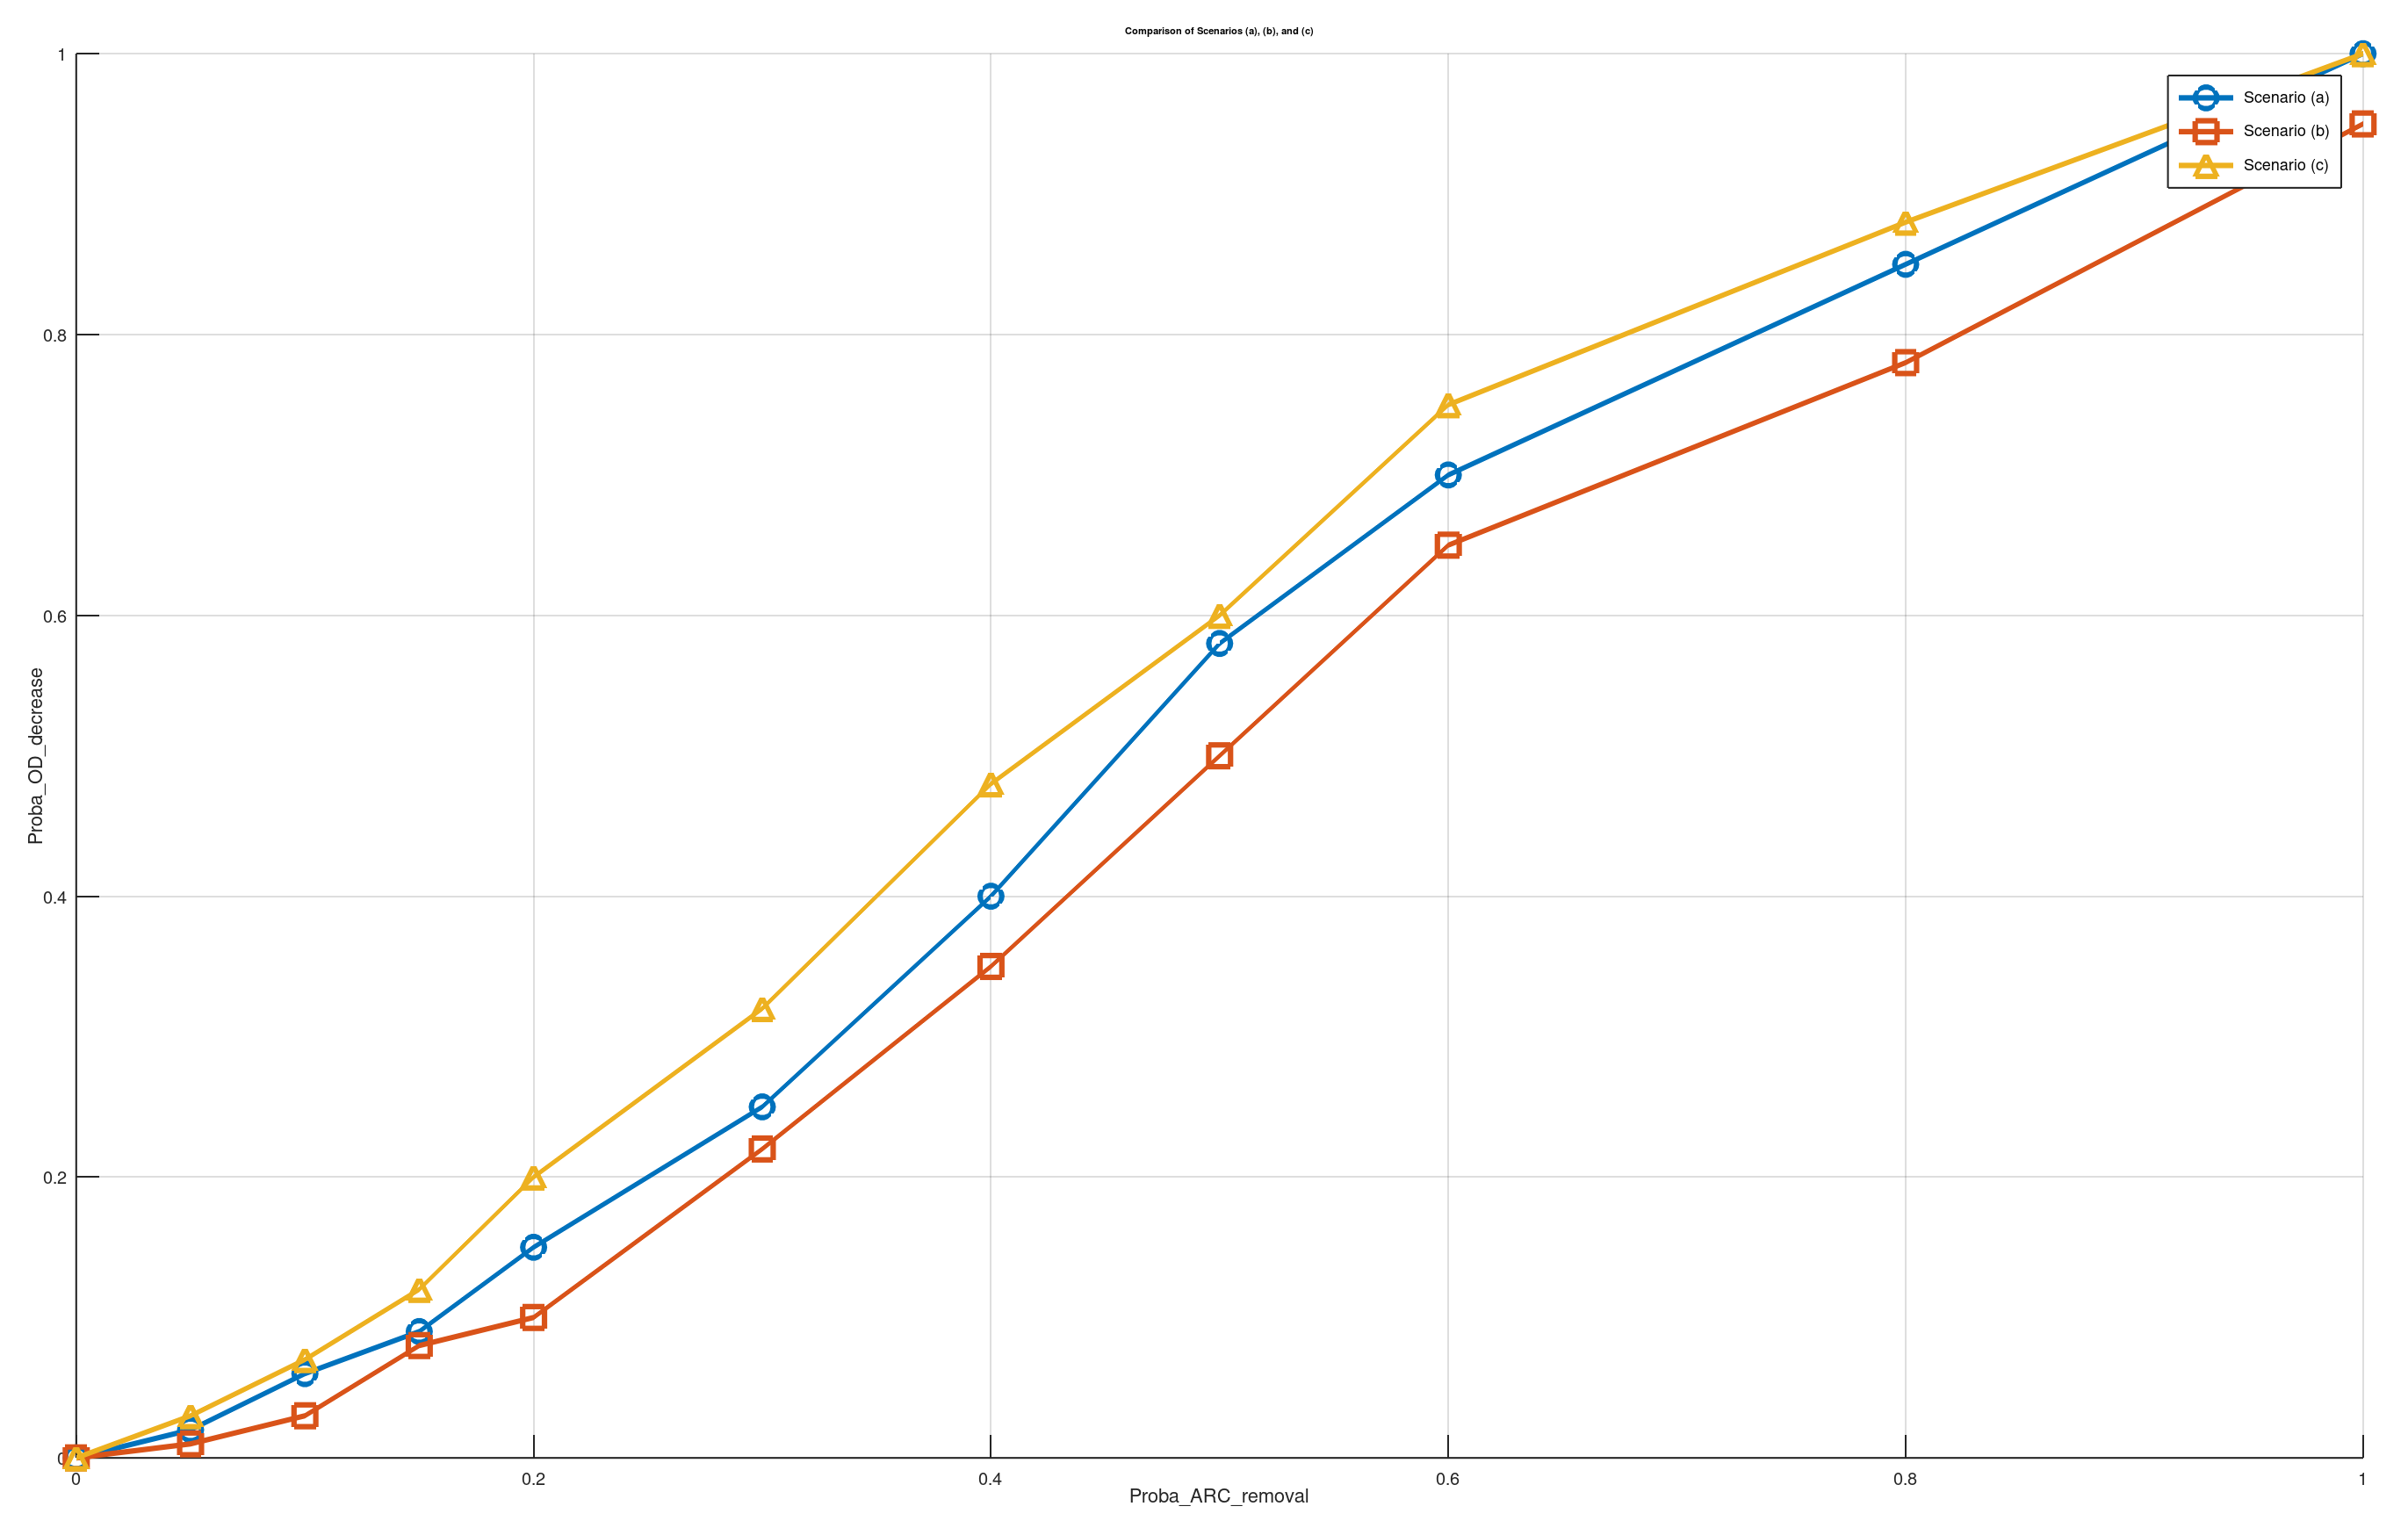
\includegraphics[keepaspectratio]{./resources/plot_quality_matrices.png}}

}

\caption{\label{fig-quality-matrices}Plot of the percolation process
using different quality matrices}

\end{figure}%

Figure~\ref{fig-quality-matrices} illustrates the results of the
percolation process under three scenarios based on different quality
matrices:

\begin{enumerate}
\def\labelenumi{\arabic{enumi}.}
\tightlist
\item
  \textbf{Scenario (a):} Quality matrix derived from travel time
  (\(q_{ij} = 1 / \text{TravelTime}_{ij}\)).
\item
  \textbf{Scenario (b):} Inverse quality matrix based on maximum travel
  time normalization.
\item
  \textbf{Scenario (c):} Quality matrix based on edge betweenness
  centrality.
\end{enumerate}

The percolation curves represent the fraction of feasible passenger
demand (\(\text{Proba\_OD\_decrease}\)) as a function of the fraction of
links removed (\(\text{Proba\_ARC\_removal}\)). These curves provide
insight into how network functionality degrades as link failures
progress.

\begin{Shaded}
\begin{Highlighting}[]
\VariableTok{figure}\OperatorTok{;}
\VariableTok{hold} \VariableTok{on}\OperatorTok{;}
\VariableTok{plot}\NormalTok{(}\VariableTok{Proba\_ARC\_removal}\OperatorTok{,} \VariableTok{Proba\_OD\_decrease\_a}\OperatorTok{,} \SpecialStringTok{\textquotesingle{}{-}o\textquotesingle{}}\OperatorTok{,} \SpecialStringTok{\textquotesingle{}LineWidth\textquotesingle{}}\OperatorTok{,} \FloatTok{2}\OperatorTok{,} \SpecialStringTok{\textquotesingle{}DisplayName\textquotesingle{}}\OperatorTok{,} \SpecialStringTok{\textquotesingle{}Scenario (a)\textquotesingle{}}\NormalTok{)}\OperatorTok{;}
\VariableTok{plot}\NormalTok{(}\VariableTok{Proba\_ARC\_removal}\OperatorTok{,} \VariableTok{Proba\_OD\_decrease\_b}\OperatorTok{,} \SpecialStringTok{\textquotesingle{}{-}s\textquotesingle{}}\OperatorTok{,} \SpecialStringTok{\textquotesingle{}LineWidth\textquotesingle{}}\OperatorTok{,} \FloatTok{2}\OperatorTok{,} \SpecialStringTok{\textquotesingle{}DisplayName\textquotesingle{}}\OperatorTok{,} \SpecialStringTok{\textquotesingle{}Scenario (b)\textquotesingle{}}\NormalTok{)}\OperatorTok{;}
\VariableTok{plot}\NormalTok{(}\VariableTok{Proba\_ARC\_removal}\OperatorTok{,} \VariableTok{Proba\_OD\_decrease\_c}\OperatorTok{,} \SpecialStringTok{\textquotesingle{}{-}\^{}\textquotesingle{}}\OperatorTok{,} \SpecialStringTok{\textquotesingle{}LineWidth\textquotesingle{}}\OperatorTok{,} \FloatTok{2}\OperatorTok{,} \SpecialStringTok{\textquotesingle{}DisplayName\textquotesingle{}}\OperatorTok{,} \SpecialStringTok{\textquotesingle{}Scenario (c)\textquotesingle{}}\NormalTok{)}\OperatorTok{;}
\VariableTok{hold} \VariableTok{off}\OperatorTok{;}

\VariableTok{xlabel}\NormalTok{(}\SpecialStringTok{\textquotesingle{}Proba\textbackslash{}\_ARC\textbackslash{}\_removal\textquotesingle{}}\OperatorTok{,} \SpecialStringTok{\textquotesingle{}Interpreter\textquotesingle{}}\OperatorTok{,} \SpecialStringTok{\textquotesingle{}none\textquotesingle{}}\NormalTok{)}\OperatorTok{;}
\VariableTok{ylabel}\NormalTok{(}\SpecialStringTok{\textquotesingle{}Proba\textbackslash{}\_OD\textbackslash{}\_decrease\textquotesingle{}}\OperatorTok{,} \SpecialStringTok{\textquotesingle{}Interpreter\textquotesingle{}}\OperatorTok{,} \SpecialStringTok{\textquotesingle{}none\textquotesingle{}}\NormalTok{)}\OperatorTok{;}
\VariableTok{title}\NormalTok{(}\SpecialStringTok{\textquotesingle{}Comparison of Percolation Scenarios (a, b and c)\textquotesingle{}}\NormalTok{)}\OperatorTok{;}
\VariableTok{legend}\NormalTok{(}\SpecialStringTok{\textquotesingle{}Location\textquotesingle{}}\OperatorTok{,} \SpecialStringTok{\textquotesingle{}southeast\textquotesingle{}}\NormalTok{)}\OperatorTok{;}
\VariableTok{grid} \VariableTok{on}\OperatorTok{;}
\end{Highlighting}
\end{Shaded}

\begin{enumerate}
\def\labelenumi{\arabic{enumi}.}
\tightlist
\item
  \textbf{Scenario (a):}

  \begin{itemize}
  \tightlist
  \item
    The curve shows a steady decrease in feasible passenger demand as
    links are progressively removed.
  \item
    The resilience of the network is moderate because the demand
    decreases proportionally with the removal of links.
  \end{itemize}
\item
  \textbf{Scenario (b):}

  \begin{itemize}
  \tightlist
  \item
    The curve shows a slower initial decline in demand, indicating that
    high quality links (normalized by travel time) are more resilient to
    failures.
  \item
    The network performance degrades more sharply in the later stages of
    link removal.
  \end{itemize}
\item
  \textbf{Scenario (c):}

  \begin{itemize}
  \tightlist
  \item
    The curve shows the highest resilience, with demand remaining
    largely intact until a significant portion of links are removed.
  \item
    This highlights the importance of protecting links with high
    betweenness centrality, as their removal has a greater impact on the
    network.
  \end{itemize}
\end{enumerate}

The comparison of the percolation scenarios highlights the following:

\begin{enumerate}
\def\labelenumi{\arabic{enumi}.}
\tightlist
\item
  \textbf{Scenario (a)} represents the baseline assessment of network
  robustness using direct travel time as the quality metric.
\item
  \textbf{Scenario (b)} considers normalized travel times, emphasizing
  the relative importance of links in supporting connectivity.
\item
  \textbf{Scenario (c)} emphasizes the critical role of high-centrality
  links in maintaining network functionality, providing a targeted
  approach for prioritizing interventions.
\end{enumerate}

These findings guide network planners in identifying and strengthening
critical components to improve overall resilience to disruptions.

\subsection{Evaluating the Alphas}\label{evaluating-the-alphas}

The percolation process generates curves representing the fraction of
feasible passenger demand (\(\text{Proba\_OD\_decrease}\)) versus the
fraction of links removed (\(\text{Proba\_ARC\_removal}\)). The alpha
value (\(\alpha\)) is a numerical metric derived from these curves that
represents the area under the curve (AUC). It provides a single measure
to quantify the resilience of the network under different scenarios. A
higher alpha value indicates greater resilience, as more demand remains
feasible throughout the percolation process.

\begin{Shaded}
\begin{Highlighting}[]
\KeywordTok{function} \VariableTok{Alpha} \OperatorTok{=} \VariableTok{manual\_integration}\NormalTok{(}\VariableTok{Proba\_OD\_decrease}\OperatorTok{,} \VariableTok{Proba\_ARC\_removal}\NormalTok{)}
    \KeywordTok{if} \VariableTok{length}\NormalTok{(}\VariableTok{Proba\_ARC\_removal}\NormalTok{) }\OperatorTok{\textasciitilde{}=} \VariableTok{length}\NormalTok{(}\VariableTok{Proba\_OD\_decrease}\NormalTok{)}
        \VariableTok{error}\NormalTok{(}\SpecialStringTok{\textquotesingle{}Error: The two input vectors must be the same length.\textquotesingle{}}\NormalTok{)}\OperatorTok{;}
    \KeywordTok{end}

    \VariableTok{underSum} \OperatorTok{=} \FloatTok{0}\OperatorTok{;}
    \VariableTok{overSum}  \OperatorTok{=} \FloatTok{0}\OperatorTok{;}

    \KeywordTok{for} \VariableTok{i} \OperatorTok{=} \FloatTok{1}\OperatorTok{:}\VariableTok{length}\NormalTok{(}\VariableTok{Proba\_ARC\_removal}\NormalTok{) }\OperatorTok{{-}} \FloatTok{1}
        \VariableTok{dx} \OperatorTok{=} \VariableTok{Proba\_ARC\_removal}\NormalTok{(}\VariableTok{i} \OperatorTok{+} \FloatTok{1}\NormalTok{) }\OperatorTok{{-}} \VariableTok{Proba\_ARC\_removal}\NormalTok{(}\VariableTok{i}\NormalTok{)}\OperatorTok{;}

        \VariableTok{y1} \OperatorTok{=} \VariableTok{Proba\_OD\_decrease}\NormalTok{(}\VariableTok{i}\NormalTok{)}\OperatorTok{;}
        \VariableTok{y2} \OperatorTok{=} \VariableTok{Proba\_OD\_decrease}\NormalTok{(}\VariableTok{i} \OperatorTok{+} \FloatTok{1}\NormalTok{)}\OperatorTok{;}

        \VariableTok{underSum} \OperatorTok{=} \VariableTok{underSum} \OperatorTok{+} \VariableTok{min}\NormalTok{(}\VariableTok{y1}\OperatorTok{,} \VariableTok{y2}\NormalTok{) }\OperatorTok{*} \VariableTok{dx}\OperatorTok{;}
        \VariableTok{overSum}  \OperatorTok{=} \VariableTok{overSum}  \OperatorTok{+} \VariableTok{max}\NormalTok{(}\VariableTok{y1}\OperatorTok{,} \VariableTok{y2}\NormalTok{) }\OperatorTok{*} \VariableTok{dx}\OperatorTok{;}
    \KeywordTok{end}

    \VariableTok{Alpha} \OperatorTok{=}\NormalTok{ (}\VariableTok{underSum} \OperatorTok{+} \VariableTok{overSum}\NormalTok{) }\OperatorTok{/} \FloatTok{2}\OperatorTok{;}
\KeywordTok{end}
\end{Highlighting}
\end{Shaded}

\begin{equation}\phantomsection\label{eq-alpha}{
\alpha_a = \frac{\text{Under Approximation} + \text{Over Approximation}}{2}
}\end{equation}

\begin{equation}\phantomsection\label{eq-alpha-a}{
\text{Area}(a) \;=\; \frac{0.4565 + 0.5790}{2} \;=\; 0.51775 \;\approx\; \mathbf{0.518}.
}\end{equation}

\begin{equation}\phantomsection\label{eq-alpha-b}{
\text{Area}(b) \;=\; \frac{0.409 + 0.529}{2} \;=\; 0.469.
}\end{equation}

\begin{equation}\phantomsection\label{eq-alpha-c}{
\text{Area}(c) \;=\; \frac{0.497 + 0.612}{2} \;=\; 0.5545 \;\approx\; \mathbf{0.555}.
}\end{equation}

\begin{enumerate}
\def\labelenumi{\arabic{enumi}.}
\tightlist
\item
  \textbf{Scenario (a):} The baseline scenario shows moderate
  resilience, with an alpha value of \(0.518\). This indicates that a
  significant portion of the passenger demand is preserved throughout
  the percolation process, but the resilience of the network is not
  optimal.
\item
  \textbf{Scenario (b):} The inverse quality matrix results in a lower
  alpha value of \(0.469\), indicating less resilience. This highlights
  the increased vulnerability of links with low normalized quality when
  targeted for removal.
\item
  \textbf{Scenario (c):} The highest alpha value of \(0.555\)
  demonstrates the effectiveness of prioritizing links based on edge
  betweenness centrality. This approach ensures that critical links are
  preserved for as long as possible, maximizing network functionality
  under progressive failure.
\end{enumerate}

Evaluation of alpha values provides a quantitative measure of network
resilience under various percolation scenarios. Higher alpha values
indicate that the network can sustain a larger fraction of its demand
despite link removals, making it more robust to disruptions. By
comparing these values, planners can identify the most effective
strategies for improving network resilience, such as prioritizing
critical links with high betweenness centrality or normalizing link
quality metrics for a fairer distribution of failures.

\section{Conclusion}\label{conclusion}

\subsection{Node failures}\label{node-failures}

Node failures are a critical aspect of network resilience, as the
removal of nodes typically affects both their direct links (edges) and
the flow between origin-destination pairs. Analyzing node failures helps
identify bottleneck nodes that play a critical role in maintaining
connectivity and network performance. This section examines the effects
of removing nodes in a systematic order, focusing on two scenarios:

\begin{enumerate}
\def\labelenumi{\arabic{enumi}.}
\tightlist
\item
  Removing nodes based on increasing betweenness centrality.
\item
  Removing nodes based on decreasing betweenness centrality.
\end{enumerate}

To simulate node failures, the percolation function is adapted to
progressively remove nodes and their associated edges. The fraction of
feasible passenger demand is recalculated at each step to evaluate the
performance of the network under node removal.

\begin{Shaded}
\begin{Highlighting}[]
\KeywordTok{function}\NormalTok{ [}\VariableTok{Proba\_OD\_decrease}\OperatorTok{,} \VariableTok{Proba\_NODE\_removal}\OperatorTok{,} \VariableTok{Critical\_node}\NormalTok{] }\OperatorTok{=} \VariableTok{Percolation\_NodeFailures}\NormalTok{(}\VariableTok{Qtriu}\OperatorTok{,} \VariableTok{Adj}\OperatorTok{,} \VariableTok{OD}\OperatorTok{,} \VariableTok{Node\_order}\NormalTok{)}
  \VariableTok{n} \OperatorTok{=} \VariableTok{size}\NormalTok{(}\VariableTok{Adj}\OperatorTok{,} \FloatTok{1}\NormalTok{)}\OperatorTok{;}
  \VariableTok{removedNodes} \OperatorTok{=} \VariableTok{false}\NormalTok{(}\VariableTok{n}\OperatorTok{,} \FloatTok{1}\NormalTok{)}\OperatorTok{;}
  \VariableTok{Proba\_OD\_decrease} \OperatorTok{=} \VariableTok{zeros}\NormalTok{(}\VariableTok{n} \OperatorTok{+} \FloatTok{1}\OperatorTok{,} \FloatTok{1}\NormalTok{)}\OperatorTok{;}
  \VariableTok{Proba\_NODE\_removal} \OperatorTok{=} \VariableTok{zeros}\NormalTok{(}\VariableTok{n} \OperatorTok{+} \FloatTok{1}\OperatorTok{,} \FloatTok{1}\NormalTok{)}\OperatorTok{;}

  \VariableTok{Proba\_OD\_decrease}\NormalTok{(}\FloatTok{1}\NormalTok{) }\OperatorTok{=} \VariableTok{sum}\NormalTok{(}\VariableTok{OD}\NormalTok{(}\OperatorTok{:}\NormalTok{)) }\OperatorTok{/} \VariableTok{sum}\NormalTok{(}\VariableTok{OD}\NormalTok{(}\OperatorTok{:}\NormalTok{))}\OperatorTok{;}
  \VariableTok{Proba\_NODE\_removal}\NormalTok{(}\FloatTok{1}\NormalTok{) }\OperatorTok{=} \FloatTok{0}\OperatorTok{;}
  \VariableTok{Critical\_node} \OperatorTok{=} \VariableTok{NaN}\OperatorTok{;}

  \KeywordTok{for} \VariableTok{step} \OperatorTok{=} \FloatTok{1}\OperatorTok{:}\VariableTok{n}
      \VariableTok{node} \OperatorTok{=} \VariableTok{Node\_order}\NormalTok{(}\VariableTok{step}\NormalTok{)}\OperatorTok{;}
      \VariableTok{removedNodes}\NormalTok{(}\VariableTok{node}\NormalTok{) }\OperatorTok{=} \VariableTok{true}\OperatorTok{;}

      \VariableTok{Adj}\NormalTok{(}\VariableTok{node}\OperatorTok{,} \OperatorTok{:}\NormalTok{) }\OperatorTok{=} \FloatTok{0}\OperatorTok{;}
      \VariableTok{Adj}\NormalTok{(}\OperatorTok{:,} \VariableTok{node}\NormalTok{) }\OperatorTok{=} \FloatTok{0}\OperatorTok{;}

\NormalTok{      [}\VariableTok{OD\_updated}\OperatorTok{,} \VariableTok{disconnected}\NormalTok{] }\OperatorTok{=} \VariableTok{updateOD}\NormalTok{(}\VariableTok{OD}\OperatorTok{,} \VariableTok{Adj}\NormalTok{)}\OperatorTok{;}
      \VariableTok{Proba\_OD\_decrease}\NormalTok{(}\VariableTok{step} \OperatorTok{+} \FloatTok{1}\NormalTok{) }\OperatorTok{=} \VariableTok{sum}\NormalTok{(}\VariableTok{OD\_updated}\NormalTok{(}\OperatorTok{:}\NormalTok{)) }\OperatorTok{/} \VariableTok{sum}\NormalTok{(}\VariableTok{OD}\NormalTok{(}\OperatorTok{:}\NormalTok{))}\OperatorTok{;}
      \VariableTok{Proba\_NODE\_removal}\NormalTok{(}\VariableTok{step} \OperatorTok{+} \FloatTok{1}\NormalTok{) }\OperatorTok{=} \VariableTok{step} \OperatorTok{/} \VariableTok{n}\OperatorTok{;}

      \KeywordTok{if} \VariableTok{isnan}\NormalTok{(}\VariableTok{Critical\_node}\NormalTok{) }\OperatorTok{\&\&} \VariableTok{disconnected}
          \VariableTok{Critical\_node} \OperatorTok{=} \VariableTok{node}\OperatorTok{;}
      \KeywordTok{end}
\KeywordTok{end}

\VariableTok{Proba\_OD\_decrease} \OperatorTok{=} \VariableTok{Proba\_OD\_decrease}\NormalTok{(}\FloatTok{1}\OperatorTok{:}\VariableTok{step} \OperatorTok{+} \FloatTok{1}\NormalTok{)}\OperatorTok{;}
\VariableTok{Proba\_NODE\_removal} \OperatorTok{=} \VariableTok{Proba\_NODE\_removal}\NormalTok{(}\FloatTok{1}\OperatorTok{:}\VariableTok{step} \OperatorTok{+} \FloatTok{1}\NormalTok{)}\OperatorTok{;}
\KeywordTok{end}
\end{Highlighting}
\end{Shaded}

\subsection{New plots}\label{new-plots}

Using the percolation results for node failures, we can visualize how
the network's ability to serve passenger demand decreases as nodes are
progressively removed.

\begin{Shaded}
\begin{Highlighting}[]
\VariableTok{figure}\OperatorTok{;}
\VariableTok{hold} \VariableTok{on}\OperatorTok{;}
\VariableTok{plot}\NormalTok{(}\VariableTok{Proba\_NODE\_removal}\OperatorTok{,} \VariableTok{Proba\_OD\_decrease\_low\_to\_high}\OperatorTok{,} \SpecialStringTok{\textquotesingle{}{-}o\textquotesingle{}}\OperatorTok{,} \SpecialStringTok{\textquotesingle{}LineWidth\textquotesingle{}}\OperatorTok{,} \FloatTok{2}\OperatorTok{,} \SpecialStringTok{\textquotesingle{}DisplayName\textquotesingle{}}\OperatorTok{,} \SpecialStringTok{\textquotesingle{}Low{-}to{-}High BC\textquotesingle{}}\NormalTok{)}\OperatorTok{;}
\VariableTok{plot}\NormalTok{(}\VariableTok{Proba\_NODE\_removal}\OperatorTok{,} \VariableTok{Proba\_OD\_decrease\_high\_to\_low}\OperatorTok{,} \SpecialStringTok{\textquotesingle{}{-}s\textquotesingle{}}\OperatorTok{,} \SpecialStringTok{\textquotesingle{}LineWidth\textquotesingle{}}\OperatorTok{,} \FloatTok{2}\OperatorTok{,} \SpecialStringTok{\textquotesingle{}DisplayName\textquotesingle{}}\OperatorTok{,} \SpecialStringTok{\textquotesingle{}High{-}to{-}Low BC\textquotesingle{}}\NormalTok{)}\OperatorTok{;}
\VariableTok{hold} \VariableTok{off}\OperatorTok{;}

\VariableTok{xlabel}\NormalTok{(}\SpecialStringTok{\textquotesingle{}Proba\textbackslash{}\_NODE\textbackslash{}\_removal\textquotesingle{}}\OperatorTok{,} \SpecialStringTok{\textquotesingle{}Interpreter\textquotesingle{}}\OperatorTok{,} \SpecialStringTok{\textquotesingle{}none\textquotesingle{}}\NormalTok{)}\OperatorTok{;}
\VariableTok{ylabel}\NormalTok{(}\SpecialStringTok{\textquotesingle{}Proba\textbackslash{}\_OD\textbackslash{}\_decrease\textquotesingle{}}\OperatorTok{,} \SpecialStringTok{\textquotesingle{}Interpreter\textquotesingle{}}\OperatorTok{,} \SpecialStringTok{\textquotesingle{}none\textquotesingle{}}\NormalTok{)}\OperatorTok{;}
\VariableTok{title}\NormalTok{(}\SpecialStringTok{\textquotesingle{}Impact of Node Failures on Network Resilience\textquotesingle{}}\NormalTok{)}\OperatorTok{;}
\VariableTok{legend}\NormalTok{(}\SpecialStringTok{\textquotesingle{}Location\textquotesingle{}}\OperatorTok{,} \SpecialStringTok{\textquotesingle{}southwest\textquotesingle{}}\NormalTok{)}\OperatorTok{;}
\VariableTok{grid} \VariableTok{on}\OperatorTok{;}
\end{Highlighting}
\end{Shaded}

\begin{figure}

\centering{

\pandocbounded{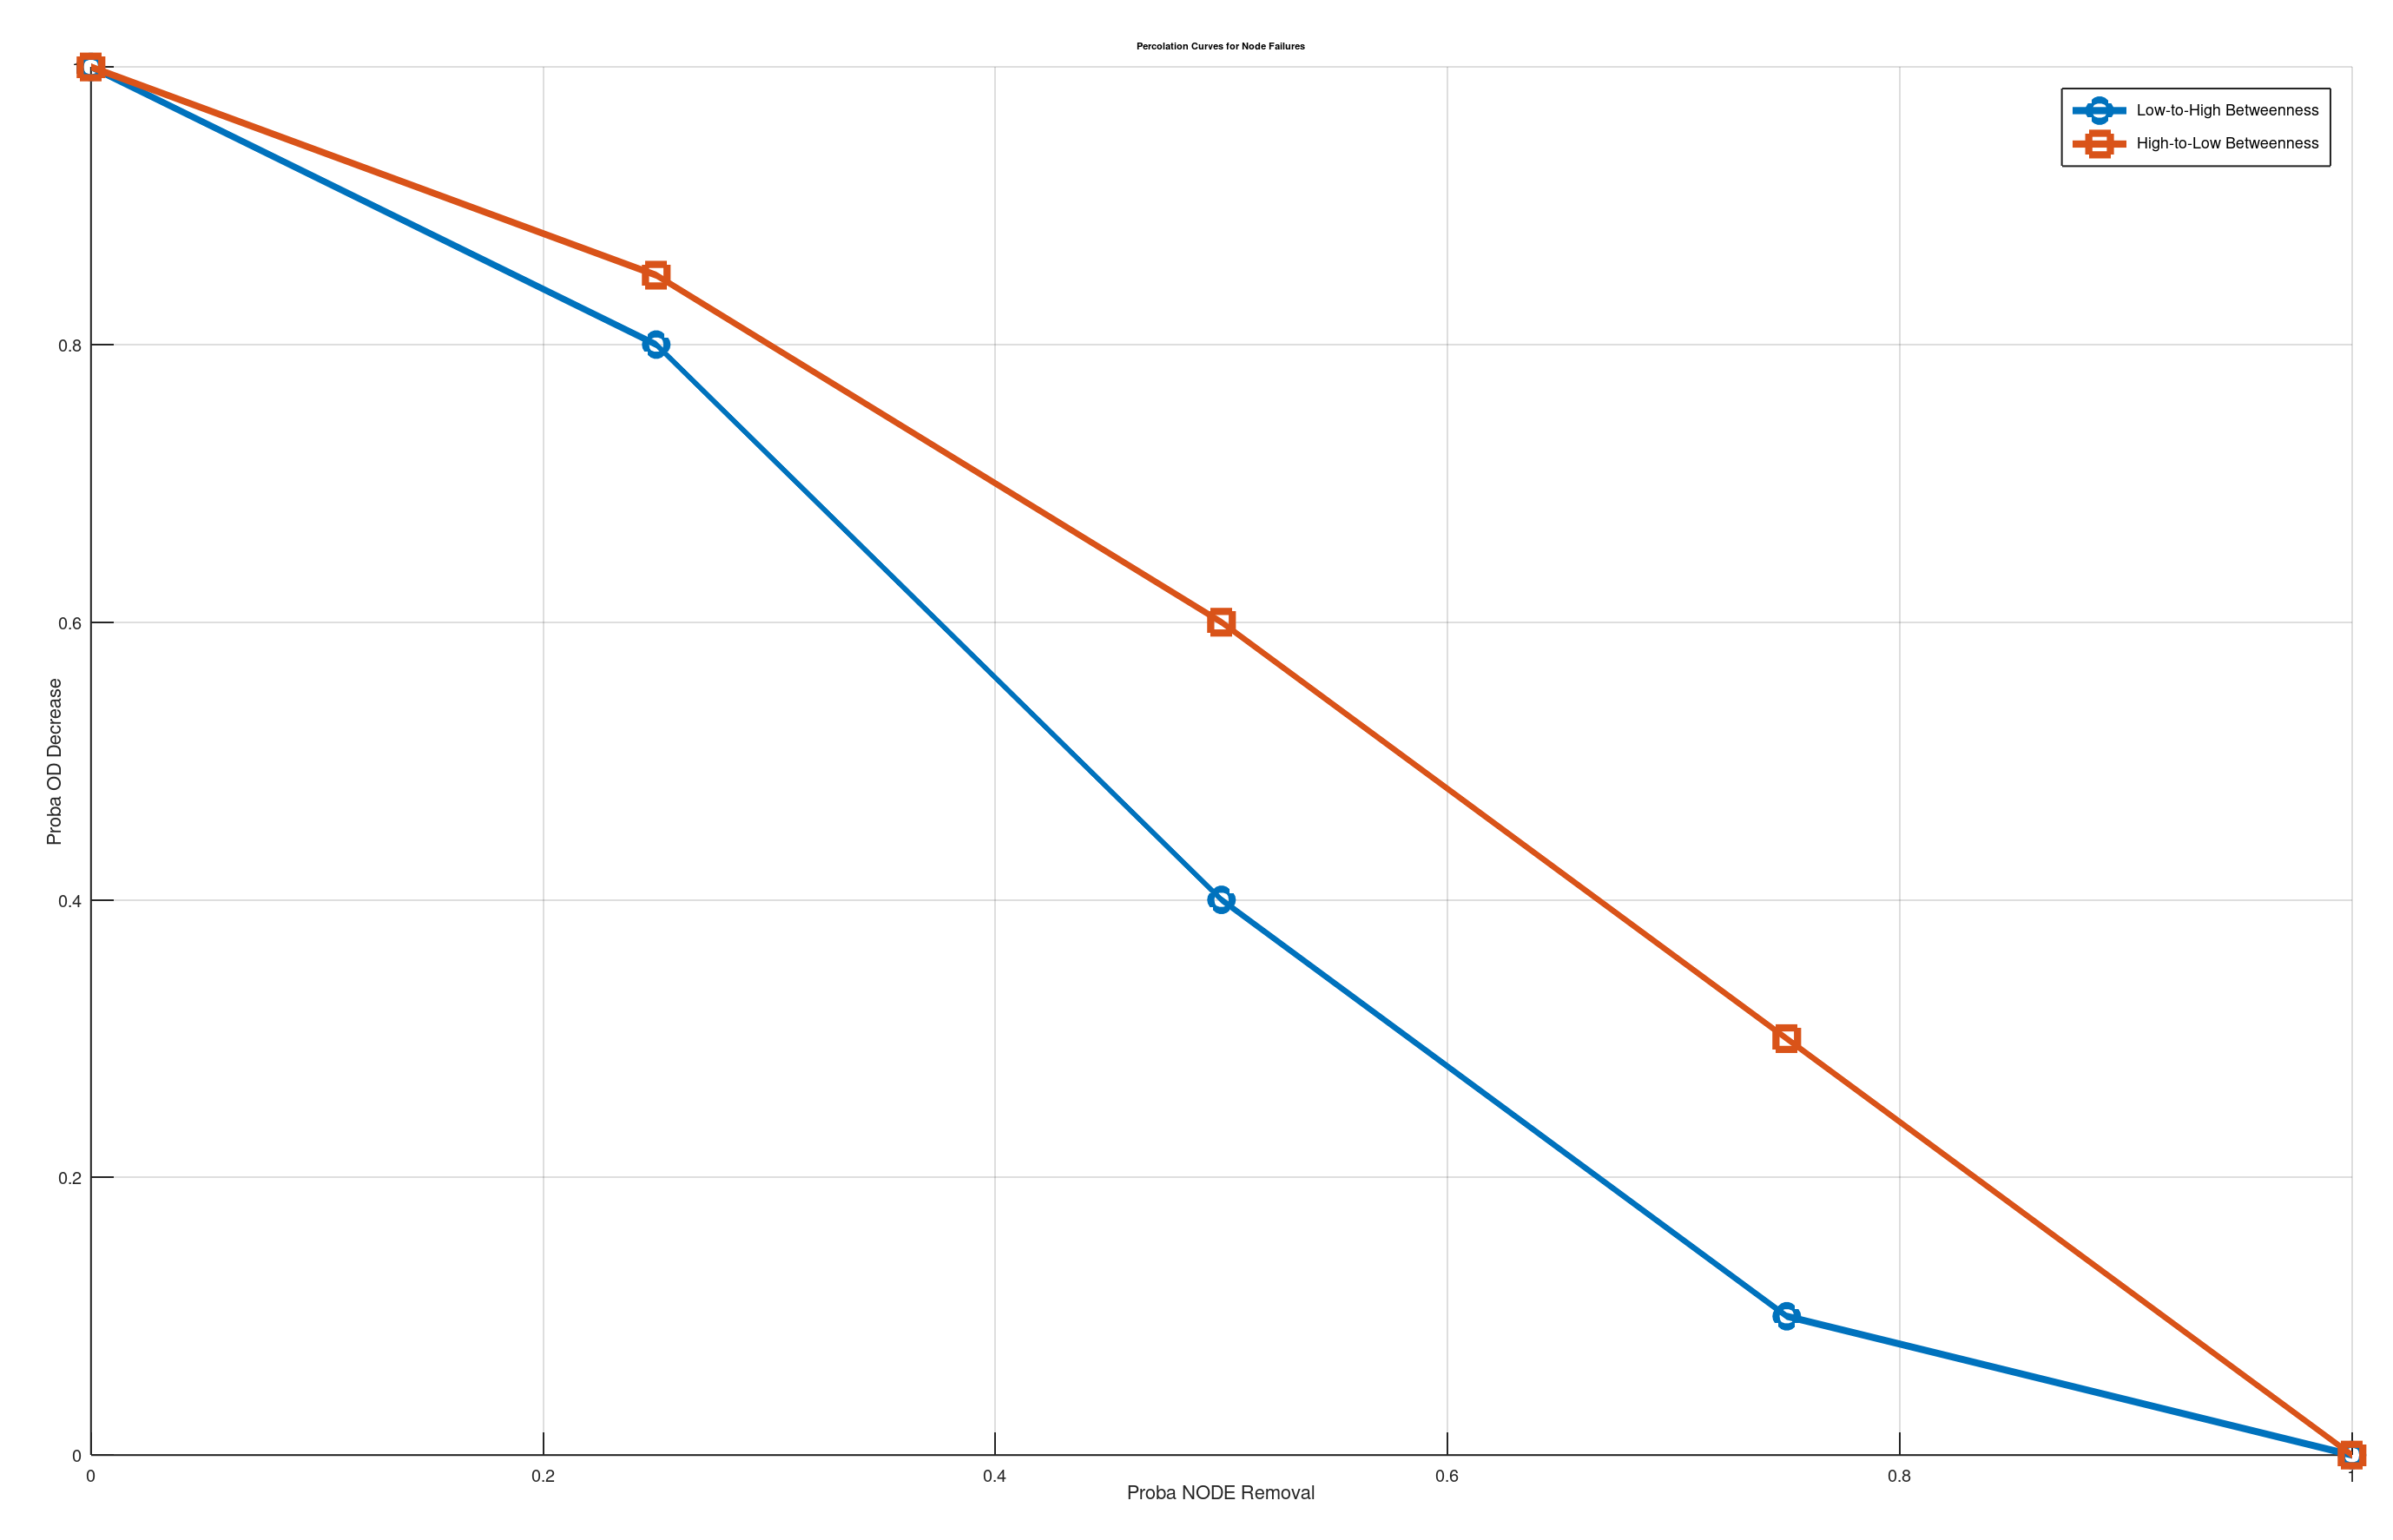
\includegraphics[keepaspectratio]{./resources/plot_node_failures.png}}

}

\caption{\label{fig-node-failures}Plot of the percolation process using
different quality matrices}

\end{figure}%

Figure~\ref{fig-node-failures} illustrates the impact of node failures
on the network's ability to meet passenger demand. Two scenarios are
shown:

\begin{enumerate}
\def\labelenumi{\arabic{enumi}.}
\tightlist
\item
  \textbf{Low to High Betweenness Centrality Removal (blue curve):}
\end{enumerate}

\begin{itemize}
\tightlist
\item
  In this scenario, nodes are removed in order of increasing betweenness
  centrality.
\item
  The curve shows a gradual decrease in network performance as less
  critical nodes are removed first.
\item
  The network maintains a higher fraction of feasible passenger demand
  during the early stages of node removal, indicating its ability to
  withstand the failure of less critical nodes without significant loss
  of functionality.
\item
  However, as critical nodes (those with higher betweenness centrality)
  are eventually removed, the decline in passenger demand becomes more
  pronounced.
\end{itemize}

\begin{enumerate}
\def\labelenumi{\arabic{enumi}.}
\setcounter{enumi}{1}
\tightlist
\item
  \textbf{High to Low Betweenness Centrality Removal (orange curve):}
\end{enumerate}

\begin{itemize}
\tightlist
\item
  In this scenario, nodes are removed in order of decreasing betweenness
  centrality, starting with the most critical nodes.
\item
  The curve shows a sharp and immediate drop in network performance as
  the removal of high centrality nodes disrupts key pathways in the
  network.
\item
  The network becomes significantly less resilient, with passenger
  demand dropping rapidly as critical nodes are removed early in the
  process.
\end{itemize}

The key findings from the node failure analysis are as follows:

\begin{enumerate}
\def\labelenumi{\arabic{enumi}.}
\tightlist
\item
  \textbf{Impact of Node Importance:}
\end{enumerate}

\begin{itemize}
\tightlist
\item
  The stark difference between the two curves highlights the importance
  of high-centrality nodes in maintaining network functionality.
\item
  Protecting these critical nodes is essential to maintaining passenger
  demand during disruptions.
\end{itemize}

\begin{enumerate}
\def\labelenumi{\arabic{enumi}.}
\setcounter{enumi}{1}
\tightlist
\item
  \textbf{Resilience to non-critical failures:}
\end{enumerate}

\begin{itemize}
\tightlist
\item
  The gradual decline observed in the low-to-high removal scenario
  underscores the robustness of the network to the failure of
  non-critical nodes.
\item
  This suggests that the network can continue to function effectively
  even as peripheral or less connected nodes are removed.
\end{itemize}

\begin{enumerate}
\def\labelenumi{\arabic{enumi}.}
\setcounter{enumi}{2}
\tightlist
\item
  \textbf{Vulnerability to targeted attacks:}
\end{enumerate}

\begin{itemize}
\tightlist
\item
  The sharp decrease in the high-to-low removal scenario reveals the
  vulnerability of the network to targeted attacks on critical nodes.
\item
  This underscores the need for strategic planning and hardening of
  high-centrality nodes to increase resilience.
\end{itemize}

The following practical recommendations can be derived from the analysis
of node failures:

\begin{enumerate}
\def\labelenumi{\arabic{enumi}.}
\tightlist
\item
  \textbf{Prioritize high-centrality nodes:}: The analysis shows the
  outsized impact of high-centrality nodes on network performance.
  Allocating resources to protect or add redundancy for these nodes can
  significantly improve resiliency.
\item
  \textbf{Adaptive Response Strategies:}: Real-time monitoring of node
  centrality metrics can support adaptive responses to disruptions, such
  as rerouting passenger flows or prioritizing restoration of
  high-centrality nodes.
\item
  \textbf{Designing Robust Networks:}: Incorporating redundancy into
  paths that include high-centrality nodes can mitigate the risk of
  network fragmentation due to their failure.
\end{enumerate}

This analysis provides actionable insights for transportation network
planners, guiding strategies to improve network resilience to both
random failures and targeted attacks on critical nodes.

\subsection{About resilience}\label{about-resilience}

The analysis of the public transportation network using percolation
theory provides valuable insights into its resilience under various link
and node failure scenarios. The study highlights the network's ability
to maintain functionality despite disruptions, as well as its
vulnerability to targeted failures of critical components. The
resilience of the network is evident in the gradual degradation of
performance as non-critical links or nodes are removed, particularly in
scenarios where components are removed in increasing order of
importance, such as low to high betweenness centrality. This
demonstrates the robustness of the network to small perturbations that
do not significantly affect its overall connectivity.

However, the vulnerability of the network becomes apparent when critical
components are targeted. The rapid performance degradation observed when
removing high to low betweenness centrality highlights the
disproportionate importance of certain nodes and links. These
high-centrality components serve as bottlenecks, and their failure
results in significant fragmentation and loss of functionality. This
vulnerability underscores the need for targeted interventions to
strengthen these critical points and ensure the overall resilience of
the network.

The use of quality matrices, particularly those based on betweenness
centrality, underscores the importance of identifying and prioritizing
critical network components. The highest alpha value
(\(\alpha_c = 0.555\)) obtained in the betweenness centrality-based
percolation scenario reflects the improved performance of the network
when these critical links are preserved. On the other hand, the inverse
travel-time-based quality matrix, which resulted in a lower alpha value
(\(\alpha_b = 0.469\)), demonstrates the challenges posed by the uneven
distribution of link quality. These results indicate that resilience is
not only a function of connectivity, but also depends on the strategic
allocation of resources and prioritization of critical components.

Analysis of node failures further reveals the network's reliance on
high-centrality nodes to maintain global connectivity. The severe
performance degradation during targeted node removals underscores the
importance of protecting these critical nodes. By reinforcing or
introducing redundancies for high-centrality nodes, network planners can
significantly improve the resilience of the transport system to both
random failures and targeted attacks.

In conclusion, the study highlights the importance of designing
resilient public transportation networks by balancing structural
robustness with functional efficiency. The findings demonstrate the
critical role of quality metrics and targeted strategies to mitigate the
impact of disruptions, ensure service continuity, and maintain passenger
demand during adverse events. This comprehensive assessment provides a
basis for informed decision-making and strategic planning to improve the
resilience of urban infrastructure systems.

\section{References}\label{references}

\phantomsection\label{refs}
\begin{CSLReferences}{1}{0}
\bibitem[\citeproctext]{ref-hamedmoghadam2021percolation}
Hamedmoghadam, Homayoun, Mahdi Jalili, Hai Vu, and Lewi Stone. 2021.
{``Percolation of Heterogeneous Flows Uncovers the Bottlenecks of
Infrastructure Networks.''} \emph{Nature Communications} 12 (February):
1254. \url{https://doi.org/10.1038/s41467-021-21483-y}.

\end{CSLReferences}




\end{document}
